\chapter{路径规划仿真试验}\label{chap:path_planning_simulation}
本章节仿真效果很多基于动画展示，不便于在论文中直接展示，相关仿真视频与源代码已上传至GitHub项目主页（\url{https://github.com/misedeshitou/ColorDynamic}）。

\section{仿真环境介绍}

本文路径规划算法的训练与测试均基于开源强化学习仿真平台 Sparrow（\url{https://github.com/XinJingHao/Sparrow-V2}）展开。Sparrow 以 Pygame 为渲染后端，在二维平面内模拟一台搭载激光雷达的差速轮式机器人，执行含动静态障碍物的点到点导航任务。其交互接口遵循标准 Gym 规范，主要包含以下三个要素：

\begin{itemize}
    \item \textbf{观测空间}：包括激光雷达的离散测距序列、机器人当前线速度与角速度，以及目标点在车体坐标系下的相对距离与航向偏角。
    \item \textbf{动作空间}：智能体输出线速度与角速度指令，支持离散和连续两种模式。
    \item \textbf{任务目标}：在含随机障碍物的动态场景中，以尽量短的路径无碰撞地到达目标点。
\end{itemize}

选用 Sparrow 的主要原因在于其训练效率高、物理建模贴近实际两点。

\subsection{训练效率}

\begin{enumerate}
    \item \textbf{并行环境（Vectorization）}：Sparrow 底层基于 PyTorch 实现，支持通过超参数 $N$ 同时运行多个独立环境副本。运动学积分、雷达模拟与碰撞检测均以批量矩阵运算的形式在 GPU 上执行，显著提升了单位时间内的样本采集量。
    \item \textbf{零拷贝数据流}：Gazebo、Webots 等传统仿真器在 CPU 端完成物理计算后，需将观测数据显式拷贝至 GPU 供网络推理，存在较大的通信开销。Sparrow 的观测张量直接在显存中生成，省去了跨设备传输步骤。
    \item \textbf{域随机化（Domain Randomization）}：每轮 reset 时，环境随机化障碍物的数量、形状、位置及运动速度，并可在雷达读数和底盘执行层面叠加高斯噪声与控制延迟，有助于提升策略的 Sim2Real 迁移能力。
\end{enumerate}

\subsection{物理建模}

\begin{enumerate}
    \item \textbf{一阶惯性运动学}：环境内置一阶低通滤波器模拟电机响应迟滞，实际速度 $V_{\text{now}}$ 的更新规则为：
    \begin{equation}
        V_{\text{now}} = K \cdot V_{\text{prev}} + (1-K) \cdot V_{\text{target}}
    \end{equation}
    即使发出较大的加减速指令，车体速度也不会瞬间跃变。本文训练时将滤波系数设为 $K=0.6$，以贴近真实电驱底盘的响应特性，同时促使策略网络学习提前减速等预判行为。
    \item \textbf{栅格化雷达模拟}：传统方法通过计算几何求射线与障碍物的交点，计算量较大。Sparrow 将障碍物编码为像素栅格，以雷达中心为原点向各方向同步扩散射线，利用 GPU 并行计算每条射线的首个遮挡距离，在保证精度的同时大幅降低了计算耗时。
\end{enumerate}

\subsection{动作空间}

针对不同算法的需求，Sparrow 提供离散与连续两种动作模式。

\subsubsection{离散动作空间}

离散模式下，动作空间共包含 8 个预设指令，覆盖前进、转弯、后退及静止等基本运动基元，适用于 DQN 等仅支持离散输出的算法，具体映射关系见表~\ref{tab:discrete_action}。

\begin{table}[H]
    \centering
    \caption{离散动作索引与对应运动指令}
    \label{tab:discrete_action}
    \begin{tabular}{llcc}
        \toprule
        \textbf{动作索引} & \textbf{运动含义} & \textbf{线速度 ($v$)} & \textbf{角速度 ($\omega$)} \\
        \midrule
        0 & 左转（小半径） & $0.2\,v_{\max}$ & $+\omega_{\max}$ \\
        1 & 左转（大半径） & $v_{\max}$ & $+\omega_{\max}$ \\
        2 & 直线前进 & $v_{\max}$ & $0$ \\
        3 & 右转（大半径） & $v_{\max}$ & $-\omega_{\max}$ \\
        4 & 右转（小半径） & $0.2\,v_{\max}$ & $-\omega_{\max}$ \\
        5 & 直线后退 & $-v_{\max}$ & $0$ \\
        6 & 微速前进 & $0.1\,v_{\max}$ & $0$ \\
        7 & 原地静止 & $0$ & $0$ \\
        \bottomrule
    \end{tabular}
\end{table}

\subsubsection{连续动作空间}

连续模式下，策略网络输出二维向量 $[a_1,\,a_2]\in[-1,1]^2$，环境按固定比例尺将其映射为底盘物理量：
\begin{itemize}
    \item 线速度：$V_l = a_1 \times 50\,\text{cm/s}$
    \item 角速度：$\omega = a_2 \times 2\,\text{rad/s}$
\end{itemize}
SAC、TransSAC 等基于连续控制的算法均采用此模式。

\subsection{DWA算法实现}
在本章的路径规划仿真中，DWA 作为传统局部规划基线，主要承担“无需训练即可部署”的对照角色。其控制量直接由速度空间搜索得到，优点是响应快、结构清晰，但由于决策完全依赖当前时刻的局部代价，遇到障碍物密集或目标方向变化较快的场景时，容易表现出路径抖动、转向保守以及绕行效率不高等问题。

从实现角度看，DWA 在 Sparrow 环境中的核心流程仍然遵循“采样--预测--评价--输出”的闭环机制：首先在给定的线速度和角速度范围内离散采样候选控制量，再通过短时前向推演得到若干条可行轨迹，随后结合目标距离、速度偏好与障碍物距离等代价项进行综合评分，最终输出当前步的最优运动指令。为了保证仿真中的连续性与安全性，本文对预测时域、障碍物硬约束和速度权重进行了针对性调优，使其能够在动态障碍物附近保持更稳妥的运动轨迹。

\subsection{DQN算法实现与离散动作基线}

DQN 在本文中承担离散动作空间下的强化学习基线任务。与 DWA 的显式代价搜索不同，DQN 通过将状态输入映射到离散动作的 Q 值分布，学习“在当前状态下应该执行哪一种动作”的策略近似，因此更适合验证奖励设计和环境建模是否合理。本文将机器人的运动命令抽象为有限个预设动作，使其能够覆盖前进、转向、后退与停止等基本控制模式，从而与环境交互形成可训练的离散决策闭环。

在训练过程中，DQN 主要依赖经验回放池和目标网络来稳定优化：一方面，经验回放打破连续采样带来的时间相关性，提高了样本利用率；另一方面，目标网络降低了 TD 目标频繁抖动造成的训练震荡，使训练过程更易收敛。由于路径规划任务中的奖励往往具有稀疏性，本文在 DQN 训练中进一步强化了进度奖励和终局奖励的区分，使智能体能够更早感知“靠近目标”和“远离障碍”的差异，避免陷入无意义的局部徘徊。

从结果上看，DQN 在训练初期的探索波动相对明显，但由于离散动作空间的约束，整体收敛过程较为平稳，适合作为与连续控制算法对比的基础模型。其不足也较为直观：离散化动作会限制轨迹平滑性，机器人在转向和减速时难以形成更细粒度的控制，因此在复杂场景中的最终路径质量通常不及连续动作算法。

\subsection{SAC算法实现与ASL框架接入}

SAC 是本文连续动作控制的核心基线算法。与 DQN 相比，SAC 直接输出连续的线速度与角速度，更适合描述机器人在路径规划中的真实运动学约束，也更容易得到平滑自然的行驶轨迹。本文采用 Actor-Critic 结构对策略和价值函数进行联合建模，其中 Actor 负责给出随机策略分布，Critic 则通过双 Q 网络对动作质量进行估计，从而缓解 Q 值高估带来的训练偏差。

在工程实现上，SAC 的训练流程与本文引入的 ASL（Actor-Learner-Sharer）框架高度适配。Actor 侧持续与环境交互并向共享经验池写入轨迹数据，Learner 则从经验池中批量采样并执行参数更新，这种解耦方式有效减少了采样与训练之间的相互阻塞，提高了系统吞吐量。对于路径规划任务而言，这一结构的实际意义在于：机器人可以在高频交互中持续积累有效样本，而网络更新则在后台稳定进行，最终形成更高的样本利用效率和更平滑的收敛曲线。

调试过程中，SAC 的主要问题集中在探索阶段的随机性偏强，以及熵系数和更新节奏对收敛速度的敏感性。为此，本文在训练中对动作幅值、奖励尺度以及更新频率进行了统一约束，使策略在前期保持足够探索、后期逐步转入稳定利用。整体来看，SAC 相比 DQN 在连续控制精度和路径平滑性上具有更明显的优势，是本文后续引入 Transformer 时采用的基础骨架。

\subsection{TransSAC算法实现与时序上下文增强}

TransSAC 是本文在 SAC 基础上的进一步增强版本，其核心思想是利用 Transformer 对历史状态序列进行编码，从而弥补标准 SAC 对短期上下文建模不足的问题。对于路径规划任务而言，机器人当前时刻的观测往往无法完整反映动态障碍物的运动趋势，尤其是在障碍物连续移动、环境反馈具有滞后性的情况下，单帧状态输入很容易导致策略出现“看见当前、忽略趋势”的局限。Transformer 的引入正是为了解决这一问题。

在实现上，本文将近期若干步的状态特征拼接为序列输入，通过自注意力机制提取其中的关键时序依赖，再将增强后的上下文特征送入 SAC 的策略网络与价值网络。这样做的直接收益是，模型不仅能判断“此刻是否安全”，还能更早捕捉障碍物的运动方向和目标区域的变化趋势，从而在决策上表现出更强的前瞻性。相比普通 SAC，TransSAC 往往在训练初期就能形成更稳定的动作偏好，路径选择也更少出现反复修正。

从训练表现来看，TransSAC 的优势主要体现在样本效率和早期收敛速度上。虽然其网络结构更复杂、单步计算开销略高，但由于时序特征提取更充分，策略可以更快建立对环境动态的稳定认知，因此在相同训练轮数下通常能获得更高的到达率和更低的平均步数。也正因如此，本文将其作为与 SAC 并列的重点对比对象，用于验证 Transformer 在路径规划强化学习中的增益。

\subsection{路径规划算法对比}
采用100次独立随机初始化的测试场景，分别评估了 DWA、SAC 和 TransSAC 三种算法在路径规划任务中的表现。评测指标包括：
\begin{itemize}
    \item \texttt{ep\_steps}：平均每回合步数

    统计\texttt{total\_steps / finished}，其中到达目标用真实步数，失败/超时按 500 次计罚。

    \item \texttt{ep\_r}：平均每回合总奖励

    统计方式是 \texttt{total\_r / finished}，统计成功回合数的平均总奖励。

    \item \texttt{arrival\_rate}：到达率

    统计100次测试场景中成功回合次数，作为到达率的百分比。

    \item \texttt{total\_score}：综合总分数

    \begin{itemize}
        \item 步数分：$\texttt{normed\_ep\_steps} = (500-\texttt{ep\_steps})/(500-70)$
        \item 奖励分：$\texttt{normed\_ep\_r} = \texttt{ep\_r}/220$
        \item 综合分：$\texttt{normed\_total\_score} = (\texttt{normed\_ep\_steps} + \texttt{normed\_ep\_r} + \texttt{arrival\_rate})/3$
    \end{itemize}
\end{itemize}

对于DWA经典算法，测试结果如下：
\begin{table}[H]
    \centering
    \caption{DWA经典算法测试结果}
    \label{tab:dwa_eval_result}
    \begin{tabular}{lcccc}
        \toprule
        \textbf{Index} & \textbf{Total Score} & \textbf{Arrival Score} & \textbf{Step Score} & \textbf{Reward Score} \\
        \midrule
        DWA & 0.304 & 0.53 & 0.442 & -0.06 \\
        \bottomrule
    \end{tabular}
\end{table}

对于强化学习算法，不同训练轮数的模型表现如下：

\begin{figure}[H]
  \centering
  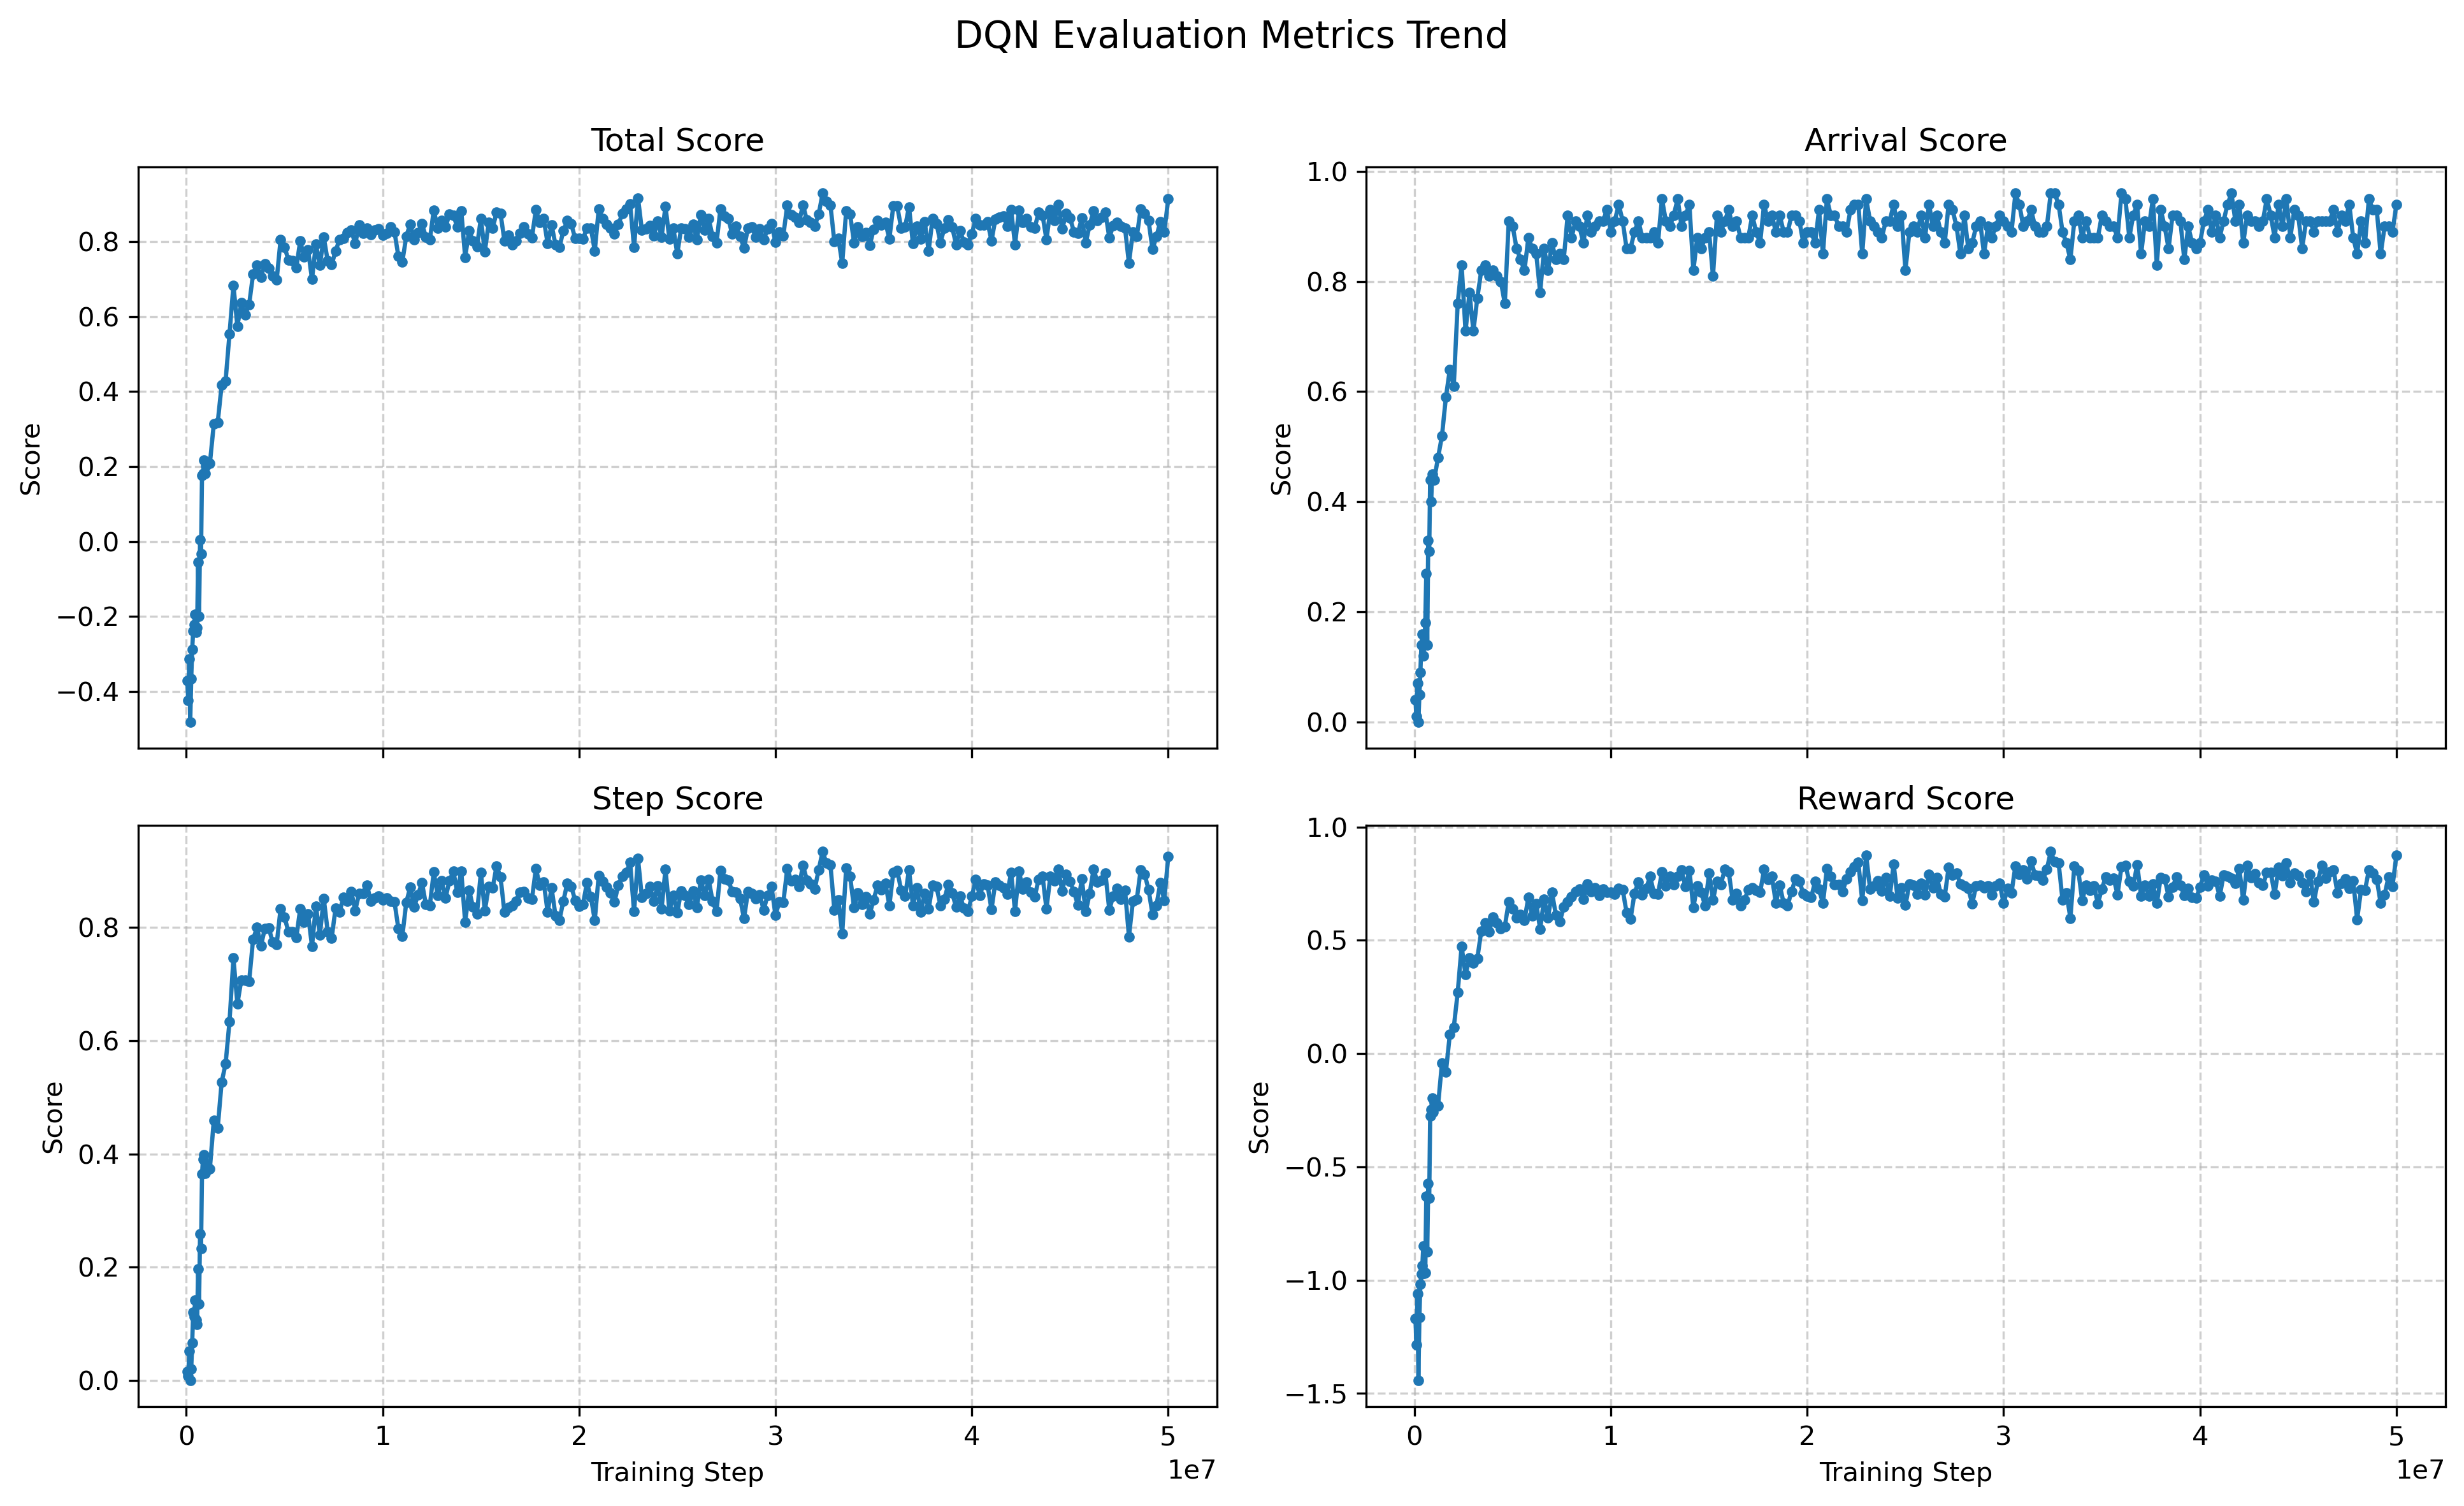
\includegraphics[width=0.7\textwidth]{figures/DQN_metrics_trend.png}
  \caption{DQN算法到达率、平均每回合步数和平均每回合奖励的训练趋势展示}
  \label{fig:dqn-showcase}
\end{figure}

\begin{figure}[H]
  \centering
  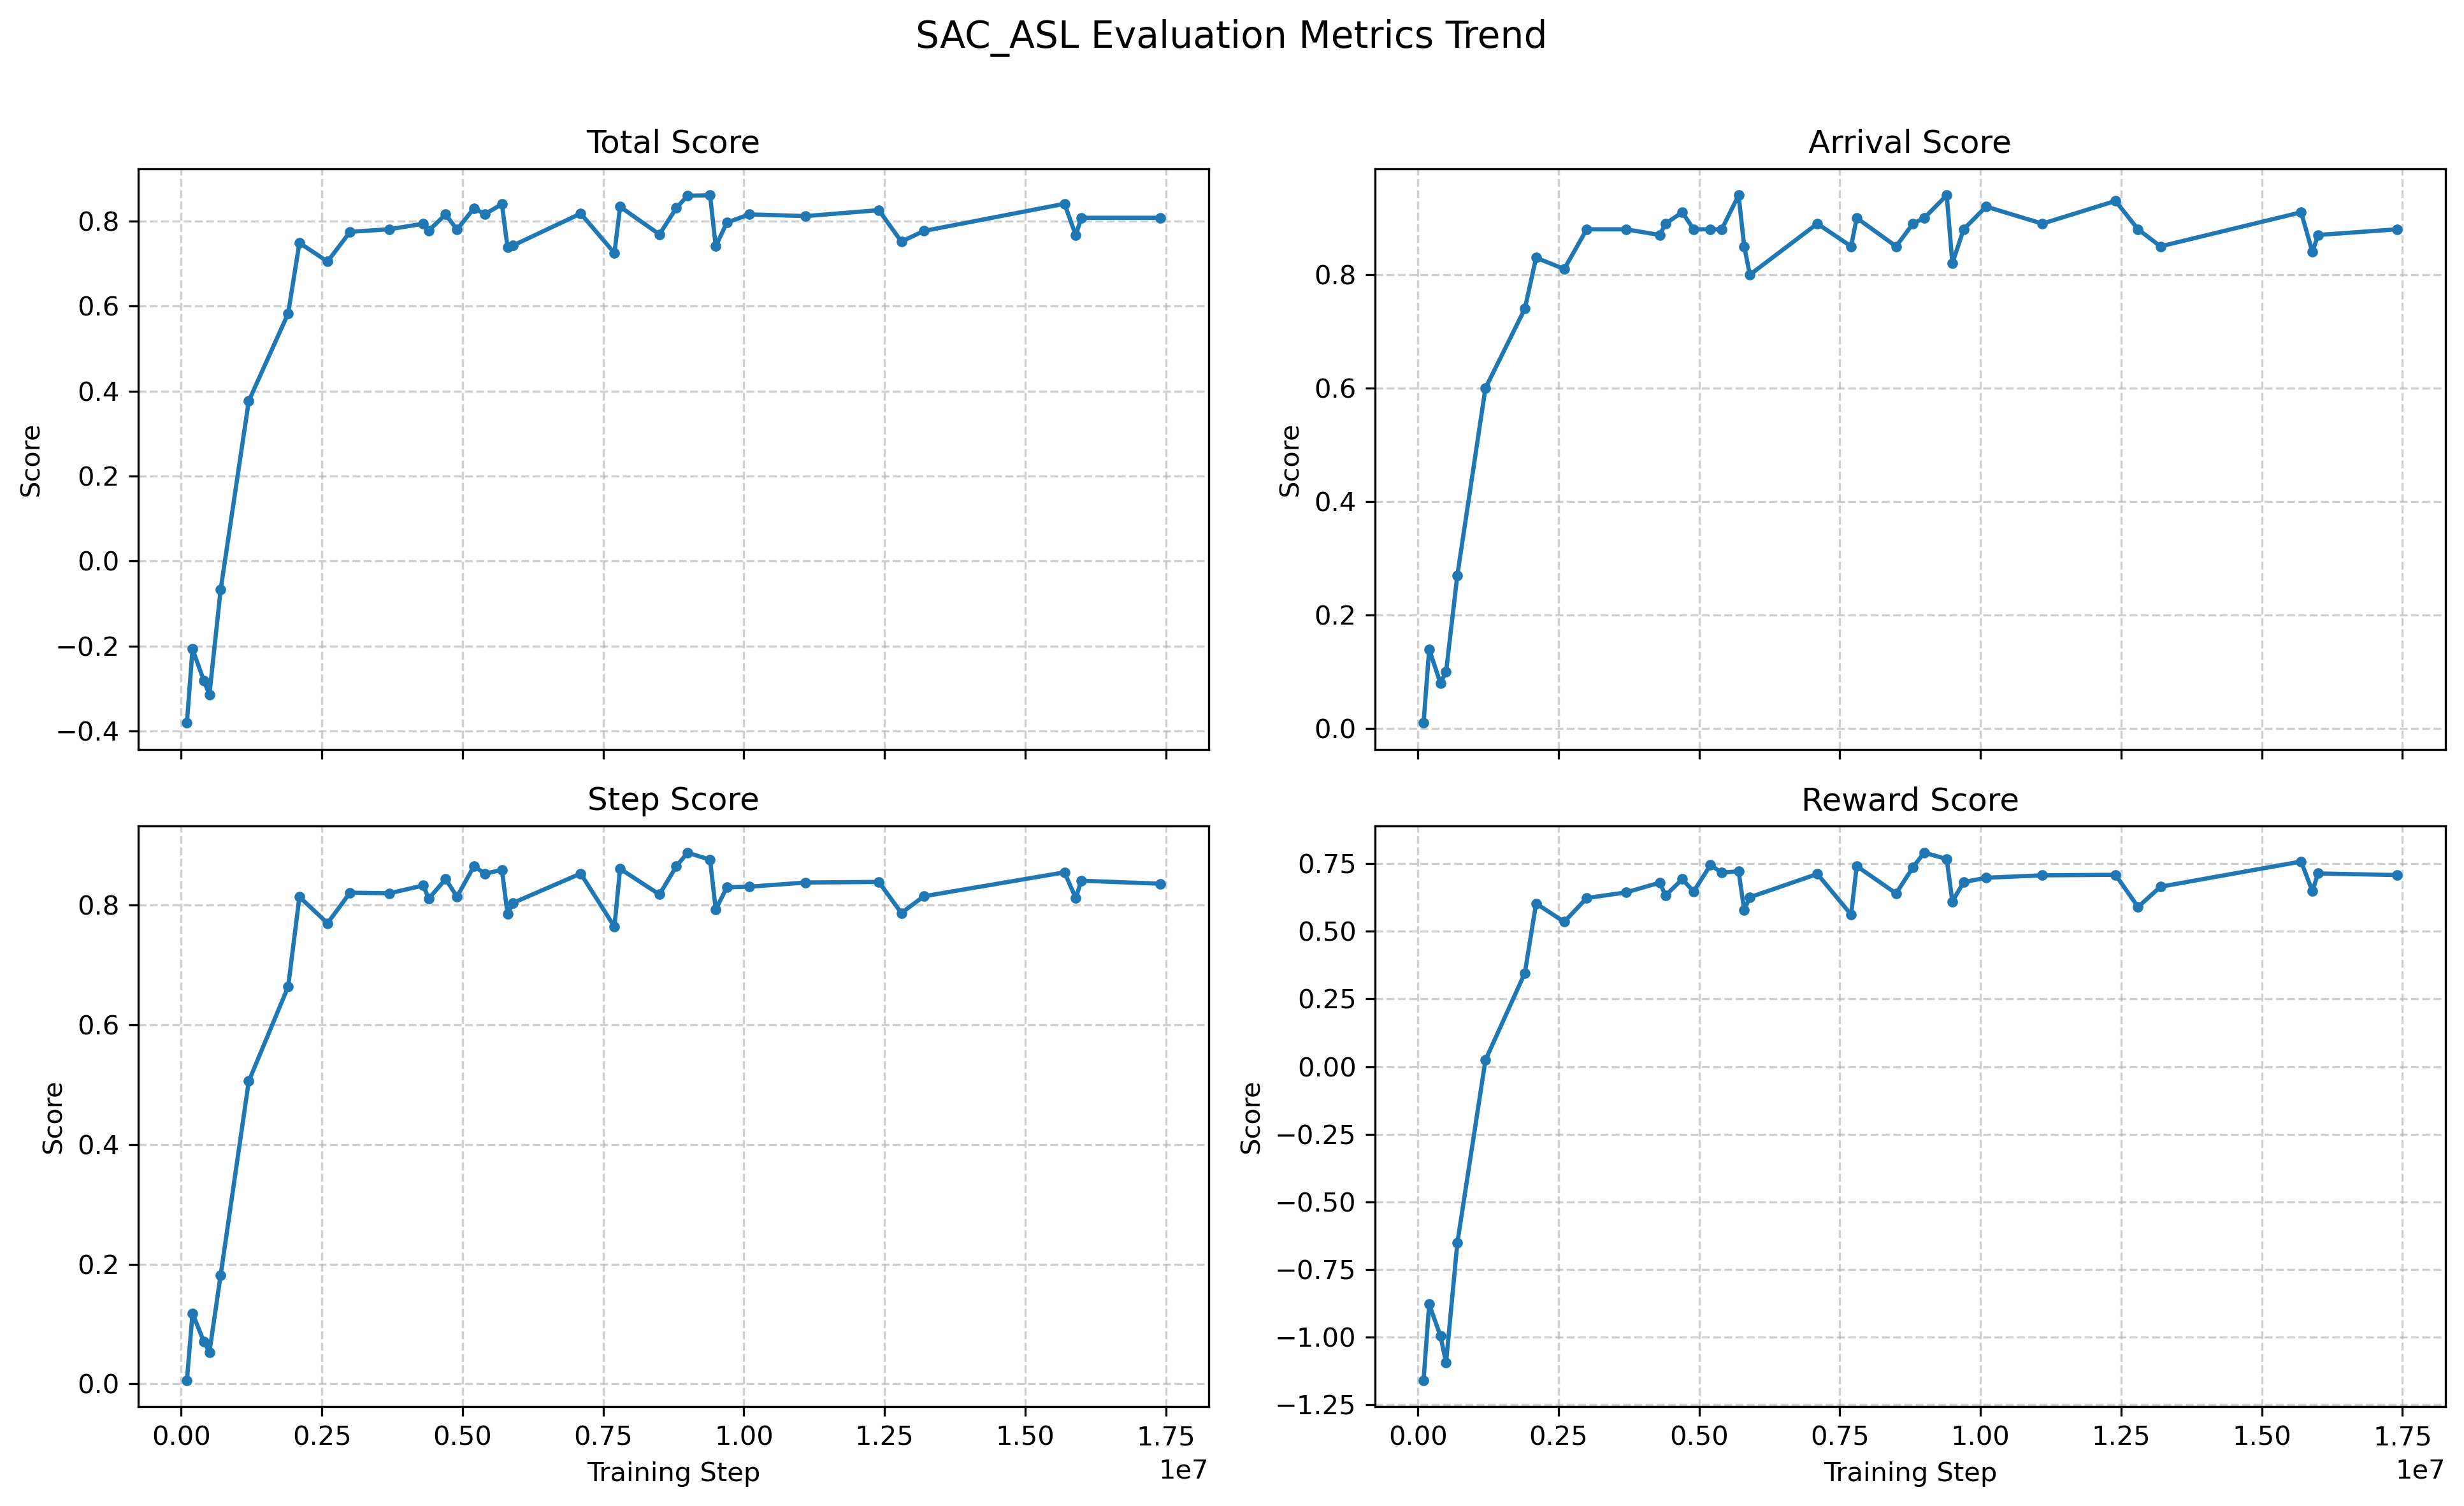
\includegraphics[width=0.7\textwidth]{figures/SAC_ASL_metrics_trend.png}
  \caption{SAC算法到达率、平均每回合步数和平均每回合奖励的训练趋势展示}
  \label{fig:sac-showcase}
\end{figure}

\begin{figure}[H]
  \centering
  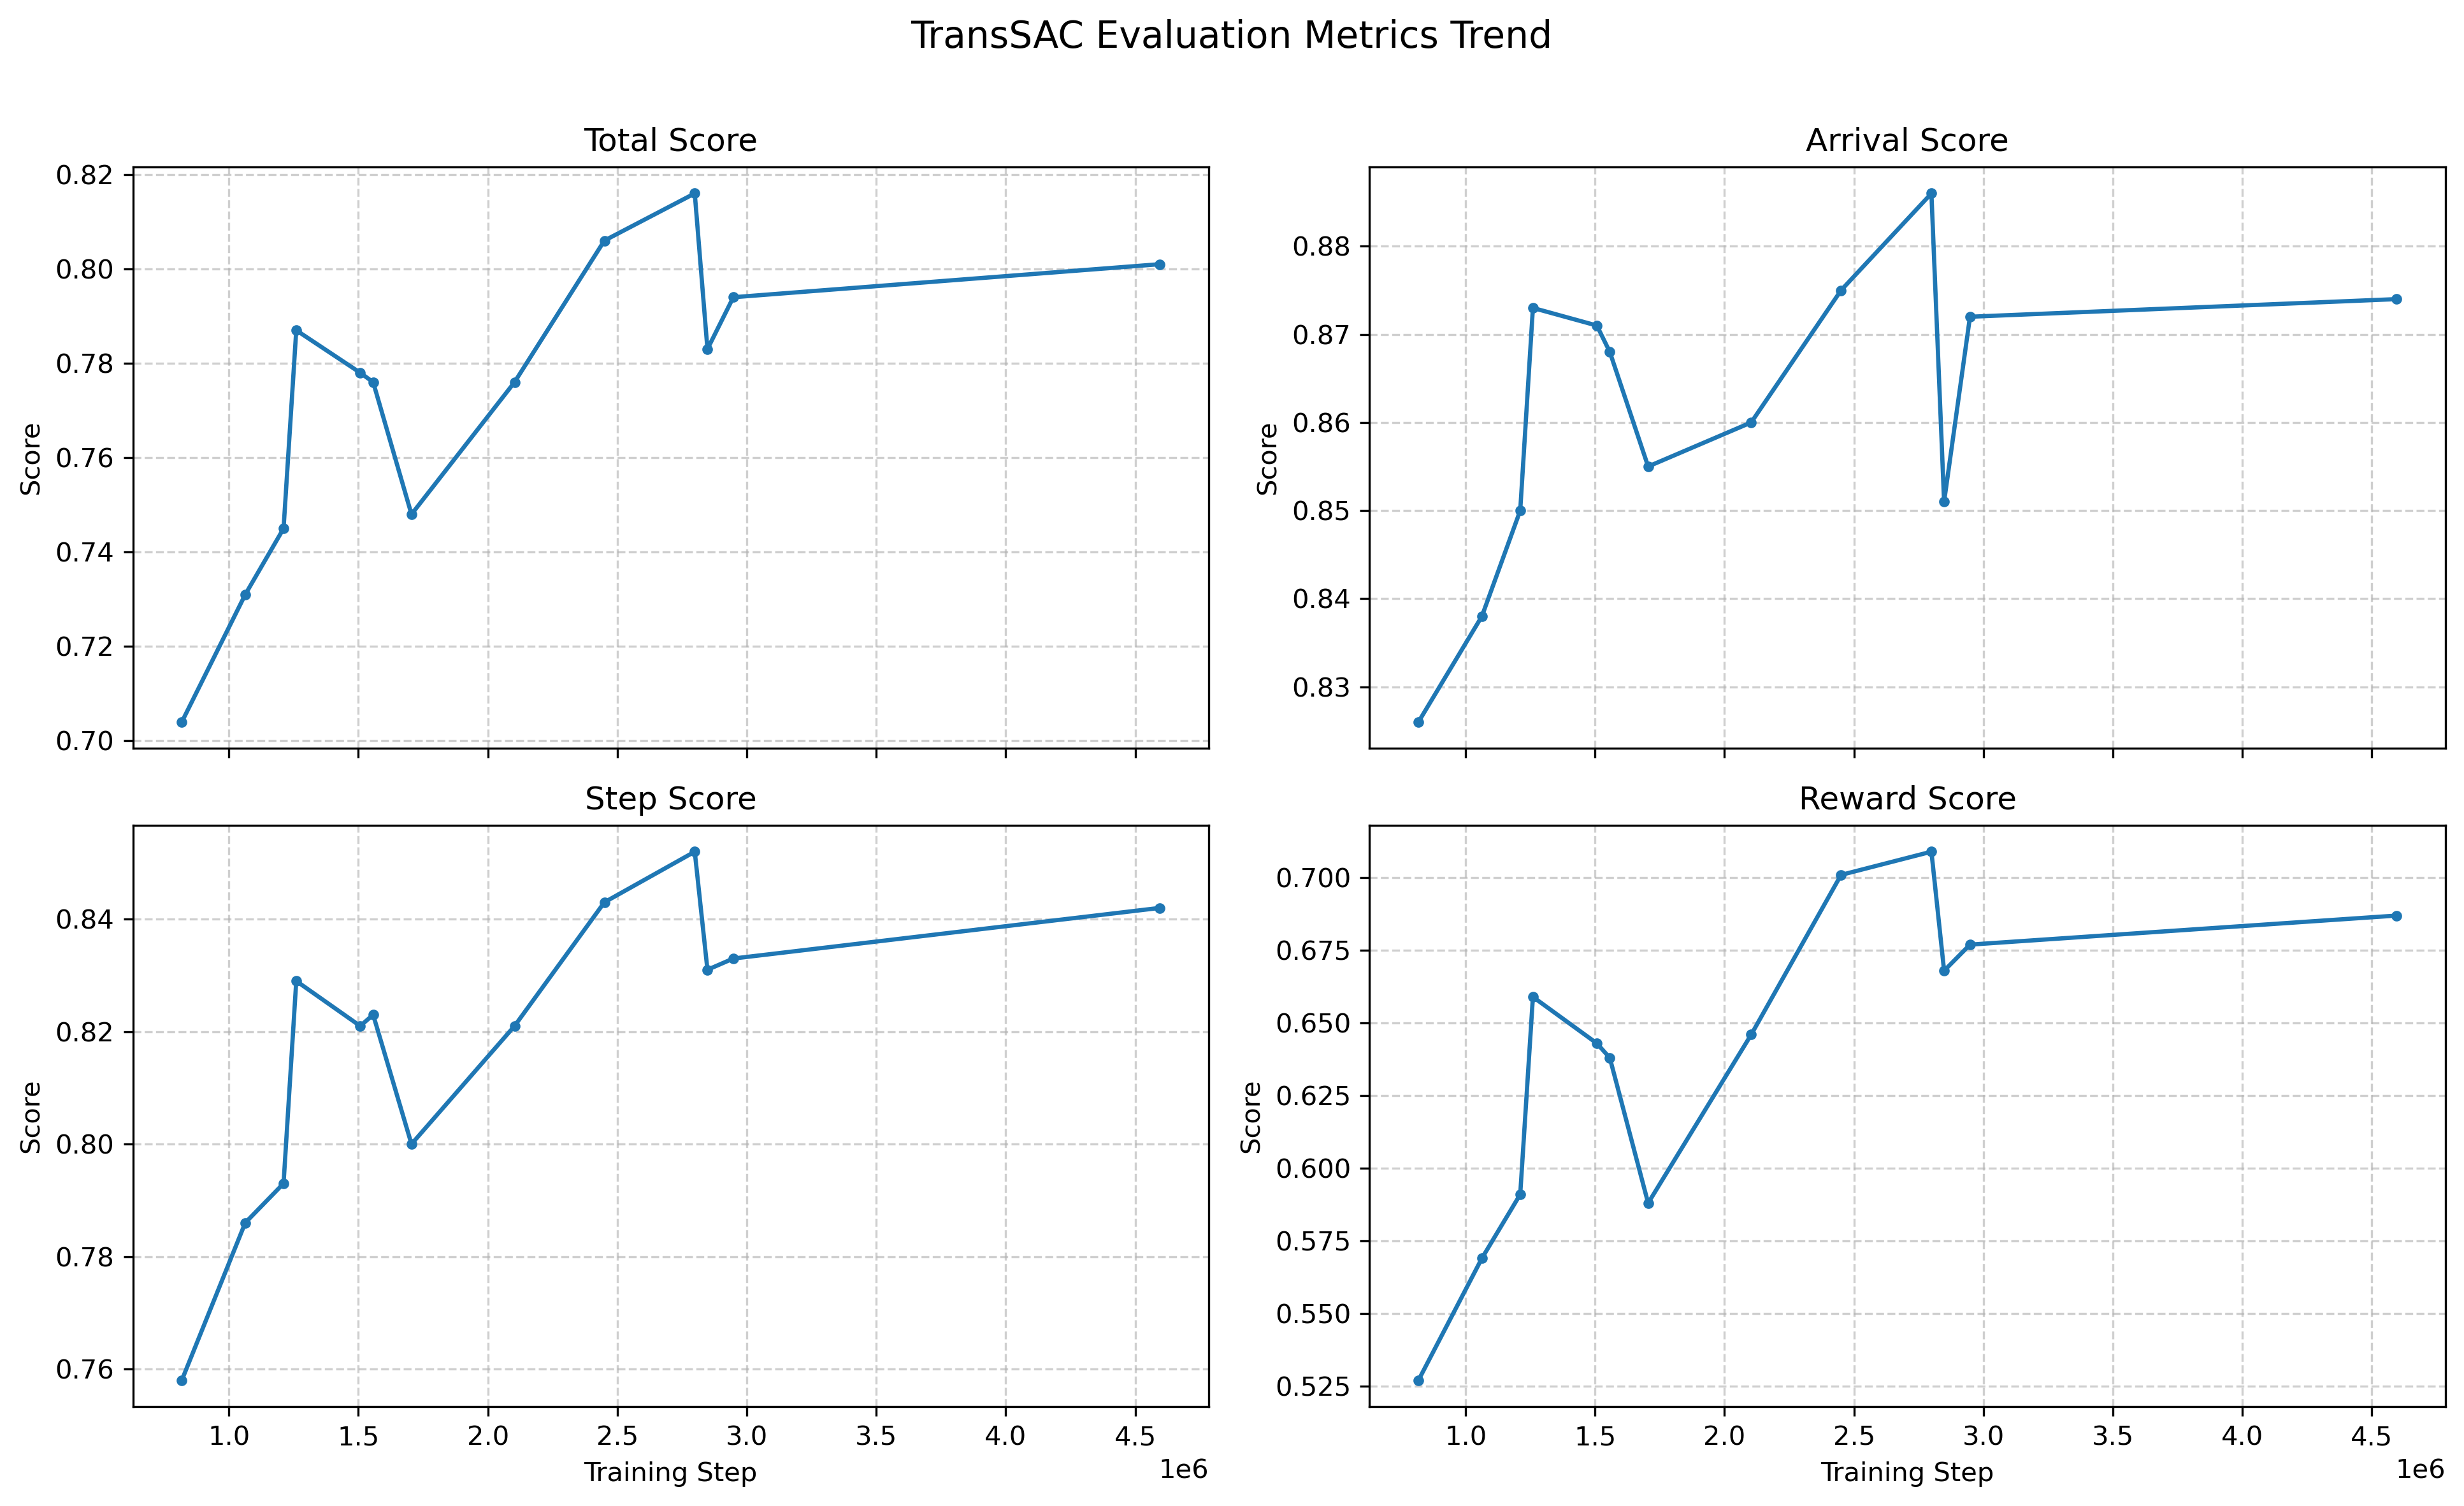
\includegraphics[width=0.7\textwidth]{figures/TransSAC_metrics_trend.png}
  \caption{TransSAC算法到达率、平均每回合步数和平均每回合奖励的训练趋势展示}
  \label{fig:transsac-showcase}
\end{figure}

由\ref{fig:dqn-showcase}和\ref{fig:sac-showcase}和\ref{fig:transsac-showcase}可以看出，DQN和SAC算
法在训练初期表现较为不稳定，平均每回合步数较多，奖励较低，到达率约为 30\%。随着训练的推进，DQN 和 SAC 的表现逐
渐提升，在 50 万步后平均每回合步数减少，奖励增加，到达率约为 85\%。两种算法在最后收敛水平、训练效率上基本相当。

而TransSAC算法在训练初期就展现出较好的性能，平均每回合步数较少，奖励较高，到达率约为 50\%。随着训练的推进，
TransSAC 的表现持续提升，在 2.5 万步即基本收敛，平均每回合步数进一步减少，奖励显著增加，到达率也约为85\%。

可以看出，引入 Transformer 结构的 TransSAC 在训练初期就展现出较好的性能，虽然最后的收敛水平与 DQN 和 SAC 
基本相当，但其训练效率和初期表现明显优于传统强化学习算法，显示了 Transformer 在强化学习中的潜力。

\begin{itemize}
    \item \textbf{平均回合步数}（$ep\_steps$）：统计成功到达目标的回合所消耗的平均步数；对于超时或碰撞失败的回合，以最大步数上限 500 步计入惩罚，以综合反映算法的导航效率。
    \item \textbf{平均回合奖励}（$ep\_r$）：统计所有回合的平均累积奖励，反映策略在奖励函数层面的综合表现。
    \item \textbf{到达率}（$arrival\_rate$）：成功抵达目标点的回合占总测试回合数的比例，是衡量算法可靠性的核心指标。
    \item \textbf{综合评分}（$normed\_total\_score$）：对上述三项指标分别归一化后取均值，计算方式如下：
\end{itemize}

\begin{equation}
\begin{aligned}
    S_{step} &= \frac{500 - ep\_steps}{500 - 70}, \quad
    S_{reward} = \frac{ep\_r}{220} \\
    S_{total} &= \frac{S_{step} + S_{reward} + arrival\_rate}{3}
\end{aligned}
\end{equation}

三种算法的测试结果汇总于表~\ref{tab:algo_comparison}。

\begin{table}[H]
    \centering
    \caption{三种路径规划算法综合性能对比}
    \label{tab:algo_comparison}
    \begin{tabular}{lcccc}
        \toprule
        \textbf{算法} & \textbf{综合评分} & \textbf{到达率} & \textbf{步数评分} & \textbf{奖励评分} \\
        \midrule
        DWA      & 0.304 & 0.530 & 0.442 & $-$0.060 \\
        SAC      & 见图~\ref{fig:sac-showcase}     & —     & —     & — \\
        TransSAC & 见图~\ref{fig:transsac-showcase} & —     & —     & — \\
        \bottomrule
    \end{tabular}
\end{table}

DWA 作为经典局部规划算法，无需训练即可部署，到达率达 53\%，但其奖励评分为负值，说明在路径质量和行驶效率方面存在明显不足，主要原因在于其基于当前时刻的局部窗口搜索，缺乏对长时序障碍物运动趋势的预判能力。

SAC 在训练初期（约 10 万步）策略尚不稳定，到达率约为 30\%；随着训练推进，策略逐步收敛，50 万步后各项指标均有显著提升。TransSAC 在 SAC 基础上引入 Transformer 序列建模模块，训练初期即表现出更高的到达率（约 50\%），50 万步后到达率超过 70\%，奖励和步数评分亦优于 SAC，体现了时序上下文建模对复杂动态场景的适应优势。

对于DWA经典算法，相关参数调优如下：
对于一个以恒定线速度 $v$ 和角速度 $\omega$ 运动的对象，其位置随时间 $t$ 的变化可写为：
\begin{equation}
\begin{aligned}
x(t) &= x_0 + \int_{0}^{t} v \cos(\theta_0 + \omega\tau) \, \mathrm{d}\tau
= x_0 + \frac{v}{\omega}\left[\sin(\theta_0 + \omega t) - \sin(\theta_0)\right],\\
y(t) &= y_0 + \int_{0}^{t} v \sin(\theta_0 + \omega\tau) \, \mathrm{d}\tau
= y_0 - \frac{v}{\omega}\left[\cos(\theta_0 + \omega t) - \cos(\theta_0)\right].
\end{aligned}
\end{equation}

\paragraph{原始离散运动模型（Euler Method）}
这是最基础的更新方式，假设在 $\Delta t$ 时间内速度和朝向恒定。
\begin{equation}
\begin{cases}
x_{k+1} = x_k + v_k \cos(\theta_k) \Delta t \\
y_{k+1} = y_k + v_k \sin(\theta_k) \Delta t \\
\theta_{k+1} = \theta_k + \omega_k \Delta t
\end{cases}
\end{equation}

\paragraph{改进后的积分运动模型（Exact Integration）}
该模型考虑了在 $\Delta t$ 时间内朝向角 $\theta$ 的连续变化（即圆弧运动）。
\begin{equation}
\begin{cases}
x(t) = x_0 + \frac{v}{\omega}(\sin(\theta_0 + \omega t) - \sin(\theta_0)) \\
y(t) = y_0 - \frac{v}{\omega}(\cos(\theta_0 + \omega t) - \cos(\theta_0)) \\
\theta(t) = \theta_0 + \omega t
\end{cases}
\end{equation}
\paragraph{改进模型的优势}
在论文论述中可从以下三个维度展开：
\begin{enumerate}
    \item \textbf{消除轨迹线性化误差}：原始离散模型默认采样周期内沿直线运动；当角速度较大或采样频率较低时，圆弧会被折线近似，从而产生几何误差。积分模型给出运动学方程的解析解，可显著降低该误差。
    \item \textbf{提高定位精度与稳定性}：在里程计（Odometry）与惯性导航中，误差会随时间累积。积分模型能降低单步预测误差，尤其在高速转弯或大角度偏转工况下可提供更准确位姿估计，从而提升滤波稳定性。
    \item \textbf{增强低频采样鲁棒性}：工程实践中采样频率可能受限（如 $10\,\mathrm{Hz}$）。相较高度依赖高频采样的离散模型，积分模型在较大时间步长 $\Delta t$ 下仍能保持较高轨迹精度。
\end{enumerate}

\subsubsection{障碍物代价函数}
\subsubsection{指数代价函数 (Soft Constraint)}

该模型采用负指数函数计算非碰撞区域的代价值，其数学表达式为：

\begin{equation}
Cost = e^{-\frac{d}{\sigma}}
\end{equation}

其中，$d$ 表示物体与障碍物之间的净距离（$net\_dist$），$\sigma$ 为平滑因子，通常取安全距离（$safe\_dist$）的三分之一。

\paragraph{逻辑设计与优势：}
\begin{itemize}
    \item \textbf{远距离衰减：} 当 $d$ 较大时，$Cost$ 趋于 $0$，表示环境对路径规划的影响极小。
    \item \textbf{近距离惩罚：} 随着 $d$ 的减小，$Cost$ 以指数级迅速增长，形成非线性惩罚。
    \item \textbf{边界平滑性：} 选取 $\sigma = \frac{safe\_dist}{3}$ 使得在 $d = safe\_dist$ 处，$Cost = e^{-3} \approx 0.049$。这种参数设计为
    机器人提供了一个平滑的避障过渡带，使其能够平滑地绕开障碍物，避免了硬约束带来的运动不连续性。
\end{itemize}

\section{DWA算法调试与局部极小值问题分析}

在动态窗口法（Dynamic Window Approach, DWA）算法的实测与部署过程中，机器人初期表现出明显的“原地打圈”现象，且设定的碰撞急停机制未能按预期生效。通过记录与分析算法运行状态，发现该现象主要源于代价函数（Cost Function）设计的不平衡以及参数配置的局部最优陷阱。

\subsection{典型异常现象：“打圈”陷阱分析}

当机器人陷入“打圈”状态时，其在评估所有可行轨迹后，认为原地旋转或远离障碍物绕圈的综合代价最低。导致这一现象的核心矛盾点可归结为以下三个方面：

\begin{itemize}
    \item \textbf{权重压制与避障过度主导：} 在前期的代价权重分配中，避障代价（Obstacle Cost）的“排斥力”远大于目标点代价（Goal Cost）的“吸引力”。只要前往目标点的路径上存在微小的碰撞风险，系统便会为了追求极低的避障代价，而放弃尝试穿过狭小空间，最终选择在原地保持较高转速（以满足速度评价指标），从而陷入局部最优。
    
    \item \textbf{长预测时域（Predict Time）的负面效应：} 在初期配置中，轨迹预测时间被设定为 $5.1\text{ s}$。在最高 $50\text{ cm/s}$ 的线速度下，系统会评估未来长达 $2.5\text{ m}$ 的运动轨迹。在密集的障碍环境中，如此长的预测轨迹在转弯时产生的“扫掠面积”极大，极易与障碍物发生干涉。为使这 $5.1\text{ s}$ 的轨迹不触碰任何障碍物，系统被迫选择曲率极大（即原地打转）的极短安全轨迹。
    
    \item \textbf{航向角代价（Heading Cost）的缺失考量：} 原始算法评价指标仅依赖轨迹末端至目标点的欧氏距离。当机器人背离目标时，为使终点靠近目标，系统可能生成倒车或大半径圆弧轨迹。由于缺乏对机身朝向目标点的显式约束，机器人在旋转过程中失去了强指向性，进一步加剧了原地绕圈的发生概率。
\end{itemize}

\subsection{动态避障策略与参数调优}

针对上述局部极小值与动态避障失效问题，经过多轮实车与仿真调试，本文对DWA算法进行了如下优化：

\subsubsection{预测时间与灵敏度的权衡}
将预测时间由 $5.1\text{ s}$ 大幅下调至 $1.0\text{ s}$，并同步降低了碰撞判断的距离阈值。该调整有效减小了轨迹的扫掠面积，提高了系统对环境的响应灵敏度。需要指出的是，预测时间不宜过小，否则会导致系统“短视”，仅在临近碰撞时才产生高代价值，从而因制动距离不足而发生实际碰撞。

\subsubsection{动静态障碍物的差异化处理机制}
实验结果表明，传统的“遇障即停”逻辑在面对动态障碍物时表现不佳，极易导致机器人陷入停滞。为此，系统舍弃了全局急停机制，转而要求机器人在动态环境中保持连续的运动能力以实现主动规避。

针对静态障碍物，为提高机器人的谨慎程度，本文采用了一种在临近区域内强制拉高代价值的硬约束策略。具体而言，当障碍物净距离 $net\_dist$ 小于等于 $15.0\text{ cm}$ 时，赋予其极高的惩罚值：
\begin{equation}
norm\_obs\_cost[net\_dist \le 15.0] = 5.0
\end{equation}
在调试中发现，若该硬性惩罚值设置过高（即梯度过大），会导致各条可行轨迹的代价差异被抹平，机器人更易倾向于停滞。因此，本文将该区域惩罚值设定为与总代价函数最大值相当的水平，且仅对静态障碍物生效，从而在保证安全性的同时维持了路径规划的平滑性。此外，考虑到引入航向角代价会大幅增加参数空间的耦合度与调优复杂度，本系统最终舍弃了该指标。

\subsection{最终参数配置}

经过上述策略的优化，机器人成功实现了鲁棒的动态避障功能。最终确定的DWA核心运动学限制与代价权重参数如表 \ref{tab:dwa_params} 所示。

\begin{table}[htbp]
    \centering
    \caption{DWA算法核心参数优化配置表}
    \label{tab:dwa_params}
    \begin{tabular}{llc}
        \toprule
        \textbf{参数变量名} & \textbf{物理意义} & \textbf{设定值} \\
        \midrule
        $max\_speed$ & 最大线速度 & $50.0 \text{ cm/s}$ \\
        $min\_speed$ & 最小线速度 & $-50.0 \text{ cm/s}$ \\
        $max\_yawrate$ & 最大角速度 & $2.0 \text{ rad/s}$ \\
        $max\_accel$ & 最大线加速度 & $2.0 \text{ m/s}^2$ \\
        $max\_dyawrate$ & 最大角加速度 & $2.0 \text{ rad/s}^2$ \\
        $v\_reso$ & 线速度搜索分辨率 & $0.1 \text{ m/s}$ \\
        $yawrate\_reso$ & 角速度搜索分辨率 & $0.2 \text{ rad/s}$ \\
        $dt$ & 控制采样周期 & $0.1 \text{ s}$ \\
        $predict\_time$ & 轨迹预测时域 & $1.0 \text{ s}$ \\
        $goal\_cost\_gain$ & 目标距离代价权重 & $0.6$ \\
        $speed\_cost\_gain$ & 期望速度代价权重 & $0.1$ \\
        $obstacle\_cost\_gain$ & 障碍物距离代价权重 & $0.3$ \\
        $robot\_radius$ & 机器人膨胀半径 & $5.0 \text{ cm}$ \\
        $safe\_dist$ & 避障预警半径 & $20.0 \text{ cm}$ \\
        \bottomrule
    \end{tabular}
\end{table}

\section{DQN算法调试}

\subsection{复合引导奖励函数设计}
强化学习中，如果只有最后到达终点才给奖励（稀疏奖励），Agent 很难学习。因此需要设计密集奖励来逐步引导策略。本文采用三类引导项：

\begin{table}[H]
    \centering
    \caption{复合引导奖励函数设计}
    \label{tab:reward_design}
    \begin{tabular}{p{0.25\textwidth}p{0.43\textwidth}p{0.24\textwidth}}
        \toprule
        \textbf{奖励项} & \textbf{方法} & \textbf{目的} \\
        \midrule
        进度 / 距离奖励  & 使用差分法计算 $\Delta d = d_{t-1} - d_t$，再除以 $v_{\max} \times \Delta t$ 并截断到 $[-1,1]$ 区间进行归一化。 & 鼓励 Agent 向目标移动，靠近目标得正分，远离扣分。 \\
        姿态 / 朝向奖励  & 计算车头朝向与“车体到目标连线”间的夹角 $\alpha$；当 $|\alpha|\in[0,0.25]$ 时给予最高 1 的朝向奖励。 & 引导机器人在靠近目标的同时保持朝向正确。 \\
        动作与动力学偏好, $R_{\mathrm{retreat\_slowdown}}$ & 根据智能体输出的线速度判断其为前进、后退或减速。 & 符合物理直觉，鼓励车辆保持合理前进速度，惩罚倒车或过慢行驶。 \\
        \bottomrule
    \end{tabular}
\end{table}

奖励的组合方式为：

\begin{equation}
    \texttt{self.reward\_vec} = 0.5 \times R_{\mathrm{distance}} + R_{\mathrm{orientation}} \times R_{\mathrm{forward}} - 0.5 \times R_{\mathrm{retreat\_slowdown}} - 0.5
\end{equation}

其中，$R_{\mathrm{orientation}} \times R_{\mathrm{forward}}$ 表示只有在前进的前提下，朝向正确才有奖励；若倒车，则无法从朝向项中获益。末尾的 $-0.5$ 是时间惩罚，使每一步都有代价，从而逼迫 Agent 尽快结束回合，避免原地徘徊刷分。

终局状态需要覆盖当前步的引导奖励：到达目标时直接将奖励赋予 \texttt{AWARD}（$+100$），碰撞或越界时直接将奖励赋予 \texttt{PUNISH}（$-100$）。这样明确标记成功与失败确保 Agent 以最终成败为优先目标。

\begin{figure}[H]
  \centering
  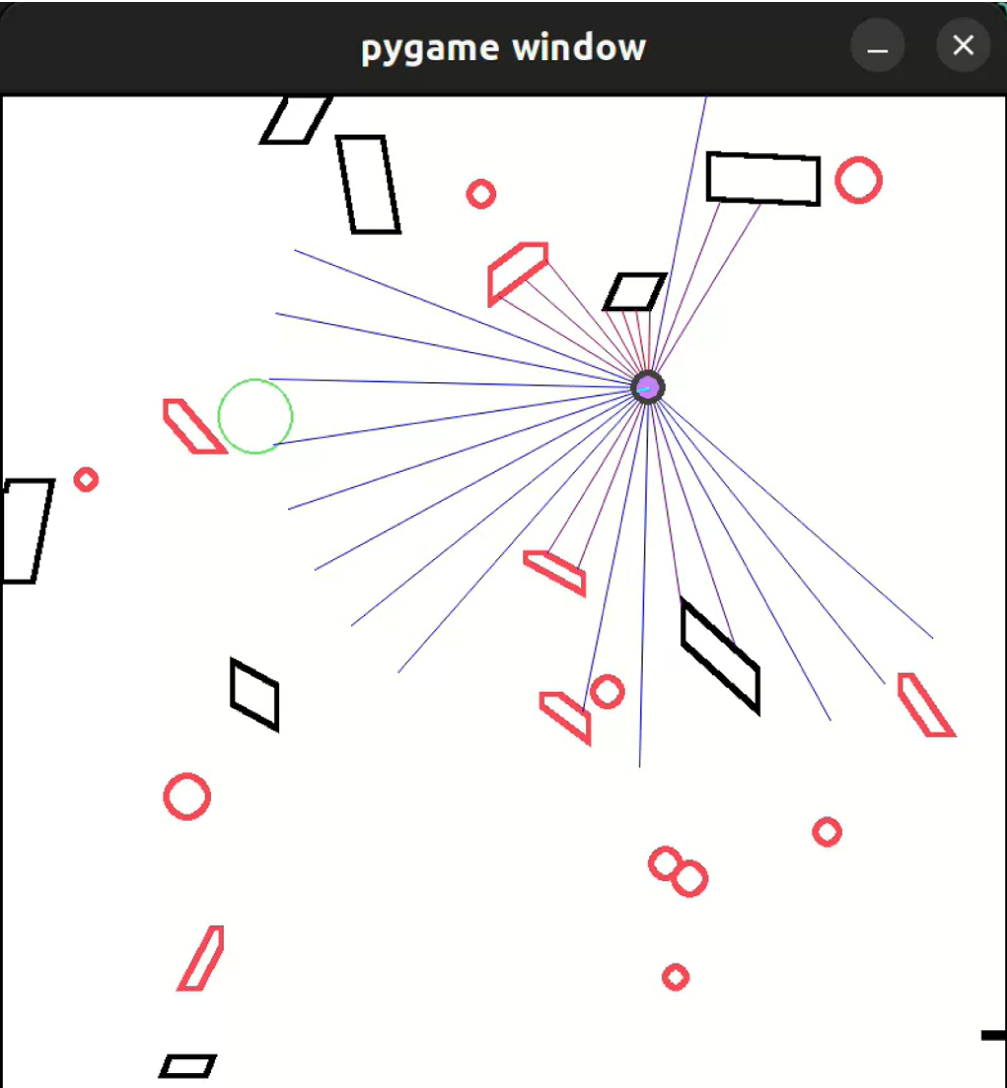
\includegraphics[width=0.5\textwidth]{figures/showcase.png}
  \caption{Sparrow环境下的路径规划仿真展示}
  \label{fig:sparrow-showcase}
\end{figure}

\section{SAC算法调试与ASL框架接入}

\subsection{分布式训练架构设计--Actor-Learner-Sharer模型}
\label{sec:shared_data_module}

\subsubsection{模块设计背景与目标}

在传统的单进程强化学习算法中，环境交互（数据采样）与神经网络更新（梯度下降）通常是串行执行的。这种同步阻塞的模式导致底层硬件算力无法得到充分利用，极大限制了算法的采样效率与收敛速度。因此需要分布式训练架构来解耦数据采集与模型训练的物理进程，从而实现真正意义上的并行加速。

\begin{tikzpicture}[
    % 定义通用样式
    task/.style={rectangle, draw=black, fill=blue!40, minimum width=2.5cm, minimum height=0.8cm, align=center},
    subtask/.style={rectangle, draw=black, fill=blue!40, minimum width=1.4cm, minimum height=0.6cm, align=center},
    cnode/.style={rectangle, draw=black, dashed, fill=gray!10, rounded corners=2pt, minimum width=2.5cm, minimum height=1.2cm, align=center},
    output/.style={rectangle, draw=black, fill=green!40!lime!60, minimum width=2.5cm, minimum height=0.6cm, align=center},
    % 定义箭头样式
    myarrow/.style={-{Stealth[scale=1.2]}, line width=3pt, draw=blue!40!gray}
]

% ====================
% (a) 单计算节点
% ====================
\node[task] (taskA) {任务};
\node[cnode, below=1cm of taskA] (nodeA) {计算节点};
\node[output, below=1cm of nodeA] (outA) {输出};

\draw[myarrow] (taskA) -- (nodeA);
\draw[myarrow] (nodeA) -- (outA);

\node[below=0.3cm of outA, font=\sffamily] {(a) 单计算节点};


% ====================
% (b) 分布式多计算节点
% ====================
\begin{scope}[xshift=8cm] % 将右侧图形整体向右平移
    
    % 上层：子任务
    \node[subtask] (sub2) {子任务2};
    \node[subtask, left=0.1cm of sub2] (sub1) {子任务1};
    \node[subtask, right=0.1cm of sub2] (sub3) {子任务3};

    % 中层：计算节点
    \node[cnode, below=1cm of sub2] (node2) {计算节点2};
    \node[cnode, left=0.3cm of node2] (node1) {计算节点1};
    \node[cnode, right=0.3cm of node2] (node3) {计算节点3};

    % 下层：输出
    \node[output, below=1cm of node2, minimum width=3cm] (outB) {输出};

    % 绘制连线
    \draw[myarrow] (sub1.south) -- (node1.north);
    \draw[myarrow] (sub2.south) -- (node2.north);
    \draw[myarrow] (sub3.south) -- (node3.north);

    \draw[myarrow] (node1.south) -- (outB.north west);
    \draw[myarrow] (node2.south) -- (outB.north);
    \draw[myarrow] (node3.south) -- (outB.north east);

    \node[below=0.3cm of outB, font=\sffamily] {(b) 分布式多计算节点};

\end{scope}

\end{tikzpicture}

为解决上述计算瓶颈与资源闲置问题，本研究引入 Actor–Learner 分布式训练架构，将环境交互（数据采样）与模型更新（参数学习）在物理进程上深度解耦，以打破算力瓶颈，大幅提高资源利用率与训练吞吐量。该架构主要包含以下三个核心部分：

\begin{enumerate}
\item \textbf{Actor（采样器）}：负责与环境进行高频交互，执行当前策略以采集经验轨迹，单步转移数据通常记录为 $(s_t, a_t, r_t, s_{t+1})$。由于仿真环境推演与逻辑判断属 CPU 密集型任务，Actor 可并行部署为大量独立进程或容器。各实例在独立的仿真环境中运行，并将采集到的数据异步写入中心经验池或以流式方式发送至 Learner。

\item \textbf{Learner（学习器）}：专注于神经网络参数的优化。Learner 从经验池中抽取小批量（Mini-batch）数据，并基于相应的损失函数（如 SAC 的 Actor-Critic 损失或 DQN 的 TD error）执行反向传播。作为 GPU/TPU 密集型任务，Learner 独占加速硬件资源，无需等待环境交互的物理步时延，从而实现极高的样本处理效率与梯度更新速率。

\item \textbf{Sharer（参数分发器）}：在大规模集群部署中常独立为参数服务组件。其主要负责全局网络权重的版本管理与分发，旨在缓解海量 Actor 同步拉取最新参数时对 Learner 计算及网络带宽造成的 I/O 瓶颈。通过高效的参数同步，Sharer 确保各 Actor 部署的策略不至于过度陈旧，严格控制 Off-policy 算法中的分布偏差（Distribution Shift）。
\end{enumerate}

\subsubsection{共享数据中枢设计}
为实现跨进程及异构硬件（CPU 与 GPU）间的高效协同，本节参考 ColorDynamic 导航系统中的相关工作 \cite{colordynamic}，设计并实现了一个高性能的共享数据中枢模块（\texttt{Shared Data Module}）。该模块扮演了连接数据采集端与模型训练端的“中央物流中枢”角色。为了彻底消除高频通信带来的 I/O 瓶颈，本系统将该模块直接部署于主内存（RAM）中，利用共享内存机制实现进程间的极速交互。该模块主要承担两大核心职能：
\begin{enumerate}
    \item \textbf{构建高速数据管道}：无阻塞地接收多 Actor 的并发经验写入，同时为 Learner 的高速迭代提供高吞吐量的随机批次采样（Batch Sampling）。
    \item \textbf{实现异步状态同步}：作为策略网络（Policy Network）参数的高速寄存器，精准协调 Learner 完成梯度更新后的参数异步下发，以及 Actor 开启新回合前的参数非阻塞拉取。
\end{enumerate}

共享数据模块扮演了连接数据采集端与模型训练端的“中央物流中枢”角色。为了消除 I/O 瓶颈，本系统将该模块部署于主内存（RAM）中，利用共享内存机制实现进程间的极速通信。

本模块的数据流转架构如图 \ref{fig:shared_data_arch} 所示：

\begin{figure}[htbp]
    \centering
\begin{tikzpicture}[
    % ==== 定义通用样式 ====
    % 基础节点样式
    basebox/.style={
        rectangle, draw=black!60, thick, rounded corners=6pt, 
        align=center, minimum height=1.8cm, text=black,
        drop shadow={opacity=0.15, shadow xshift=1.5mm, shadow yshift=-1.5mm}
    },
    % 特定节点样式（带微渐变）
    buffer/.style={basebox, top color=blue!5, bottom color=blue!15, minimum width=4.8cm},
    register/.style={basebox, top color=orange!5, bottom color=orange!15, minimum width=4.8cm},
    actorbox/.style={basebox, top color=green!5, bottom color=green!15, minimum width=5cm},
    learnerbox/.style={basebox, top color=red!5, bottom color=red!15, minimum width=5cm},
    % 箭头样式
    data_arrow/.style={-{Stealth[scale=1.2]}, line width=1.5pt, draw=blue!70!gray, text=black!80},
    weight_arrow/.style={-{Stealth[scale=1.2]}, line width=1.5pt, draw=orange!80!red, text=black!80},
    % 共享内存背景样式
    shared_mem/.style={
        rectangle, draw=black!40, dashed, thick, rounded corners=10pt, 
        fill=gray!8, inner sep=18pt
    }
]

% ==== 1. 定义顶部节点 (Shared Memory 内部) ====
\node[buffer] (buffer) {
    \textbf{向量化环形经验池} \\
    \fontsize{9pt}{10pt}\selectfont \sffamily (Ring Replay Buffer) \\
    \vspace{2pt}
    \fontsize{8pt}{9pt}\selectfont \ttfamily \color{black!70} [s, a, r, s', dw] \sffamily 异构张量存储
};

\node[register, right=2.5cm of buffer] (register) {
    \textbf{模型参数寄存器} \\
    \fontsize{9pt}{10pt}\selectfont \sffamily (Actor Policy Weights) \\
    \vspace{2pt}
    \fontsize{8pt}{9pt}\selectfont \ttfamily \color{black!70} [actor\_param] \sffamily 字典状态字典
};

% ==== 2. 绘制共享数据中枢背景框 ====
\begin{scope}[on background layer]
    \node[shared_mem, fit=(buffer) (register)] (shared) {};
    % 背景框的标题
    \node[anchor=south, font=\bfseries\sffamily\large, text=black!80, yshift=4pt] 
        at (shared.north) {Shared Data 通信中枢 (主内存 RAM)};
\end{scope}

% ==== 3. 定义底部节点 ====
\node[actorbox, below=3.5cm of buffer] (actor) {
    \textbf{Actor 进程} \small (数据采集端) \\
    \vspace{2pt}
    \fontsize{9pt}{10pt}\selectfont \sffamily \color{black!70} (运行于 CPU 或 推理 GPU)
};

\node[learnerbox, below=3.5cm of register] (learner) {
    \textbf{Learner 进程} \small (模型训练端) \\
    \vspace{2pt}
    \fontsize{9pt}{10pt}\selectfont \sffamily \color{black!70} (运行于 高性能 GPU)
};

% ==== 4. 绘制数据流转箭头 ====

% (1) Actor -> Buffer (写入经验)
\draw[data_arrow] (actor.north) -- (buffer.south) 
    node[midway, left=4pt, font=\sffamily\small] {写入转移经验};

% (2) Learner -> Register (更新权重)
\draw[weight_arrow] (learner.north) -- (register.south) 
    node[midway, right=4pt, font=\sffamily\small] {更新权重};

% (3) Buffer -> Learner (采样批次数据 - 交叉线)
% 使用 pos 参数调整文字位置，并添加白色背景避免线条穿过文字
\draw[data_arrow] (buffer.315) -- (learner.135) 
    node[pos=0.25, right=4pt, font=\sffamily\small, fill=white, inner sep=2pt, rounded corners=2pt] {采样批次数据};

% (4) Register -> Actor (拉取最新权重 - 交叉线)
\draw[weight_arrow] (register.225) -- (actor.45) 
    node[pos=0.25, left=4pt, font=\sffamily\small, fill=white, inner sep=2pt, rounded corners=2pt] {拉取最新权重};

\end{tikzpicture}
\caption{分布式 Actor-Learner 共享数据流转架构图}
\label{fig:shared_data_arch}
\end{figure}

\subsubsection{核心数据结构设计}

为充分满足大规模分布式强化学习中的并发读写与异构设备协同需求，本模块在底层数据结构设计上遵循以下两项核心原则：（1）向量化存储以适应并行采样；（2）异构设备感知的透明映射以消除数据流转的物理瓶颈。

\paragraph{向量化环形缓存池（Vectorized Ring Buffer）}

在本架构中，Actor 端并行部署 $N$ 个独立的仿真环境进行同步采样。若采用传统二维经验池 $(Max\_Size, Feature\_Dim)$，则需对 $N$ 个环境的数据依次拼接后写入，这会引入高频的列表操作与内存重排开销。为此，本模块将经验回放池升级为三维张量结构 $\mathcal{D} \in \mathbb{R}^{Max\_Size \times N \times State\_Dim}$，使得 $N$ 个环境的采样数据可在底层以矩阵块的形式原子写入，避免了序列化与重新索引的计算浪费。

同时，为防止内存占用的无限增长，该缓存池采用环形覆盖机制。系统维护一个循环写入指针 $ptr$，每当新数据写入时自动递增；当 $ptr$ 达到 $Max\_Size$ 时通过取模运算 $ptr \leftarrow ptr \bmod Max\_Size$ 自动回卷至缓存起始位置，新样本覆盖最旧的数据。这一设计既保证了数据的"热"性（确保 Learner 采样自相对新鲜的转移），又严格将内存峰值锁定在预分配的上界，避免了动态扩展带来的GC延迟。

\paragraph{三端异构硬件自适应映射（Tri-Device Memory Mapping）}

在实际部署中，数据流通涉及三类计算设备：Actor 端推理设备（CPU 或推理 GPU，记为 $A\_dvc$）、中心存储设备（主内存 RAM，记为 $B\_dvc$）、Learner 端训练设备（高性能 GPU，记为 $L\_dvc$）。若在数据入库与采样的每个环节都手动管理这些设备间的张量转移，会引入繁冗的代码耦合与难以预测的内存碎片化。

为此，本模块在初始化时显式配置这三类设备标识，在执行 $\texttt{Add}()$ 与 $\texttt{Sample}()$ 等核心操作时自动调用 PyTorch 的设备无关接口（如 $\texttt{.to}(device)$）。具体地，当 Learner 调用 $\texttt{Sample}()$ 方法时，系统先从主内存批量读取数据，随后在返回前自动将其转移至 $L\_dvc$，使调用方无需感知底层的设备寻址细节。

\begin{algorithm}
\caption{共享数据中枢的异构张量流转与自旋锁控制伪代码}
\label{alg:shared_data}
\textbf{输入}: 采集端设备 $A\_dvc$ (CPU), 训练端设备 $L\_dvc$ (GPU), 经验池容量 $Max\_Size$, 批次大小 $B$\\
\textbf{初始化}: 
\begin{itemize}
    \vspace{-0.2cm}
    \item 预分配主存 ($RAM$) 经验池张量 $\mathcal{D} \in \mathbb{R}^{Max\_Size \times N \times State\_Dim}$
    \item 初始化自旋锁状态矩阵 $busy \leftarrow [\text{False}, \text{False}]$
    \item 队列写入指针 $ptr \leftarrow 0$
\end{itemize}
\vspace{-0.2cm}
\begin{algorithmic}[1]
\Function{Add}{$transition\_data$} \Comment{由 Actor 并发调用，位于 $A\_dvc$}
    \While{$busy[1] == \text{True}$} \Comment{轻量级自旋锁等待}
        \State \text{Pass} 
    \EndWhile
    \State $busy[1] \leftarrow \text{True}$ \Comment{获取经验池锁}
    \State $\mathcal{D}[ptr] \leftarrow transition\_data$ \Comment{数据存入主内存}
    \State $ptr \leftarrow (ptr + 1) \pmod{Max\_Size}$ \Comment{环形队列覆写机制}
    \State $busy[1] \leftarrow \text{False}$ \Comment{释放锁}
\EndFunction

\State
\Function{Sample}{} \Comment{由 Learner 高频调用，意图用于 $L\_dvc$}
    \While{$busy[1] == \text{True}$} 
        \State \text{Pass} 
    \EndWhile
    \State $busy[1] \leftarrow \text{True}$
    \State $batch \leftarrow \text{RandomSelect}(\mathcal{D}, B)$ \Comment{从主内存抽取小批量数据}
    \State $busy[1] \leftarrow \text{False}$
    
    \State $batch\_L \leftarrow batch\mathbf{.to}(L\_dvc)$ \Comment{\textbf{底层隐式设备映射}}
    \State \Return $batch\_L$ \Comment{返回的张量已原生驻留于 GPU}
\EndFunction
\end{algorithmic}
\end{algorithm}

\subsubsection{并发控制与轻量级读写锁机制}

在多进程共享内存架构中，并发访问冲突是系统性能的关键制约。若 Learner 在执行参数寄存器写操作时，某个 Actor 同时尝试读取该参数，将导致张量内存被破坏。更严重的是，如果采用传统的全局互斥锁（Mutex），会强制所有竞争线程进入阻塞态并触发昂贵的内核态上下文切换，这对纳秒级别的张量访问操作而言开销巨大。

针对此问题，本系统设计了细粒度自旋锁机制以替代系统级锁。核心思想是：维护一个状态向量 $\texttt{busy} \in \{\text{False}, \text{False}\}$，其中 $\texttt{busy}[0]$ 保护"模型参数寄存器"的读写，$\texttt{busy}[1]$ 保护"经验池"的读写。这种细粒度分离使得数据域与权重域的竞争可以独立控制，大幅降低了全局锁阻塞的概率。

更重要的是，当某进程发现目标锁已被占用时，不是挂起等待（开销 $\sim 100\,\mu s$），而是进入紧密自旋轮询状态（轮询周期 $\sim 10^{-4}\,s$）。鉴于张量操作通常耗时极短（$< 1\,ms$），短期轮询的开销远小于线程被唤醒的延迟，从而实现"busy-waiting 优于阻塞等待"的场景。同时，虽然自旋会消耗 CPU 周期，但由于 Learner 与 Actor 运行于不同物理核心，这种消耗不会竞争 GPU 计算资源，反而能充分利用多核的计算平面。

当双端进程竞争同一把锁（例如 Actor 和 Learner 同时尝试访问经验池）时，自旋锁机制使未获取锁的进程进入 \texttt{while True} 的高频轮询状态（休眠 $10^{-4}$ 秒级别），而非挂起等待。由于张量转移操作耗时极短，这种短效轮询机制在保证绝对数据安全的同时，将等待开销降到了最低。

\begin{figure}[H]
  \centering
  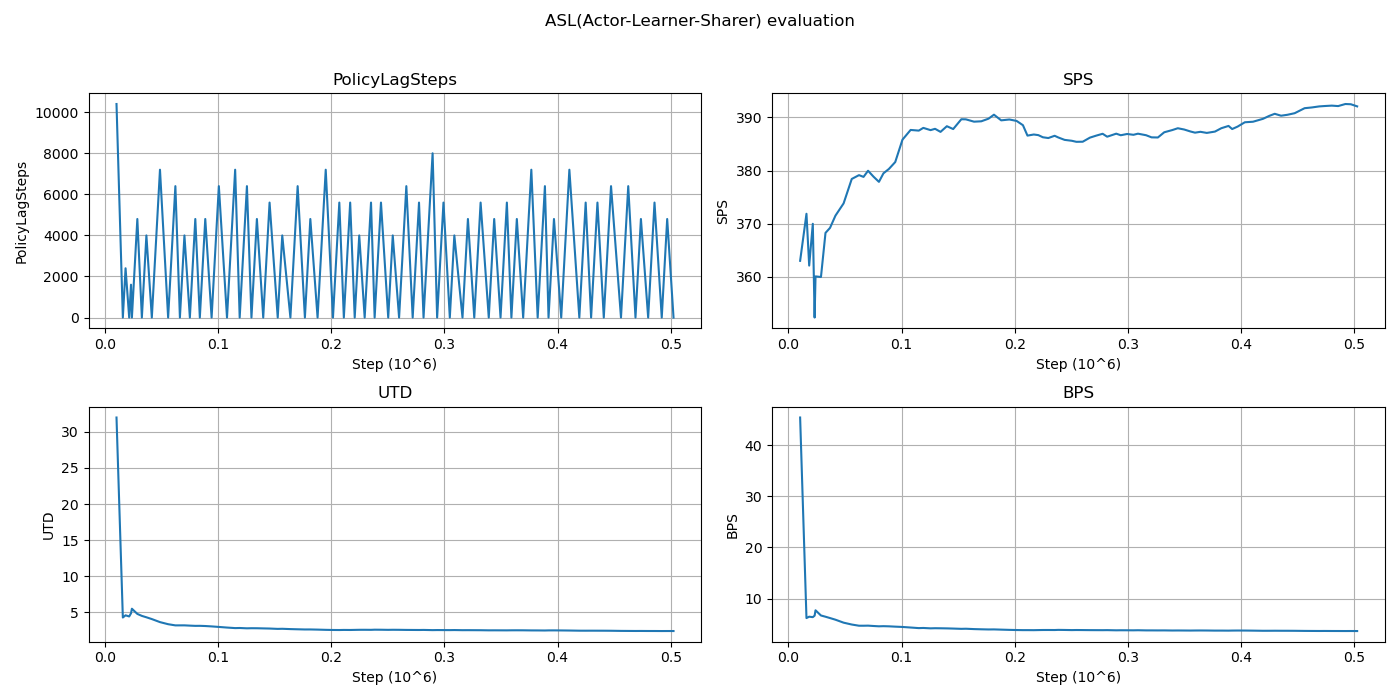
\includegraphics[width=0.9\textwidth]{figures/ASL_analysis.png}
  \caption{ASL架构性能分析}
  \label{fig:ASL-analysis}
\end{figure}
在分布式强化学习训练中，系统吞吐量、资源利用率与组件通信延迟是评估架构有效性的核心指标。图\ref{fig:ASL-analysis}给出了 Actor-Learner-Sharer（ASL）架构在 50 万步（$0.5 \times 10^6$ steps）训练周期内的性能曲线。结合曲线形态，可归纳为以下三点：
\begin{enumerate}
    \item 高效且解耦的并发吞吐量 (SPS \& BPS 分析)
    ASL 架构的核心优势在于通过 Sharer（共享经验池）将数据采样（Actor）与梯度计算（Learner）进行物理与逻辑上的解耦。

    \begin{itemize}
        \item 数据采样率 (SPS - Steps Per Second): 图中 SPS 曲线在训练初期经历短暂的预热后，迅速攀升并稳定在 380 至 390 之间。这表明 Actor 进程组能够以极高的效率持续与环境进行交互。SPS 的稳步微升进一步证明了环境重置或缓存机制在长期运行中表现出良好的鲁棒性，未出现阻塞或内存泄漏等衰减现象。
        \item 批处理更新率 (BPS - Batches Per Second): Learner 的 BPS 曲线在训练极早期（探索期）处于高位，随后迅速下降并稳定在 4 左右的水平。SPS 与 BPS 的独立稳定运行，有力证明了 ASL 架构成功打破了传统单进程 RL 中“采样等训练，训练等采样”的同步木桶效应，实现了 CPU（环境推理）与 GPU（梯度反向传播）算力的满载流水线作业。
    \end{itemize}

    \item 稳定的数据更新比 (UTD 分析)
    UTD (Update-To-Data Ratio) 定义了网络更新次数与环境交互步数的比例，是控制强化学习训练节奏的关键超参数。

    \begin{itemize}
        \item 如图所示，UTD 曲线的形态与 BPS 高度一致，在经过初始的陡降后，长程稳定在较低的数值区间（约 2 至 3 左右）。
        \item 学术意义： 这种低且稳定的 UTD 设定是针对异策略（Off-policy）算法（如 SAC）的典型优良特征。它保证了 Learner 不会因为过度消费旧数据而导致过拟合（Overfitting）或 Q 值高估，同时 Actor 源源不断地注入高新鲜度的数据，维持了探索与利用（Exploration vs. Exploitation）的动态平衡。
    \end{itemize}

    \item 异步通信与容忍延迟 (PolicyLagSteps 分析)
    策略延迟（PolicyLagSteps）是衡量分布式架构通信开销与策略陈旧度（Staleness）的最关键指标，它记录了 Actor 当前使用的采样策略落后于 Learner 最新策略的步数。

\end{enumerate}

\begin{figure}[H]
  \centering
  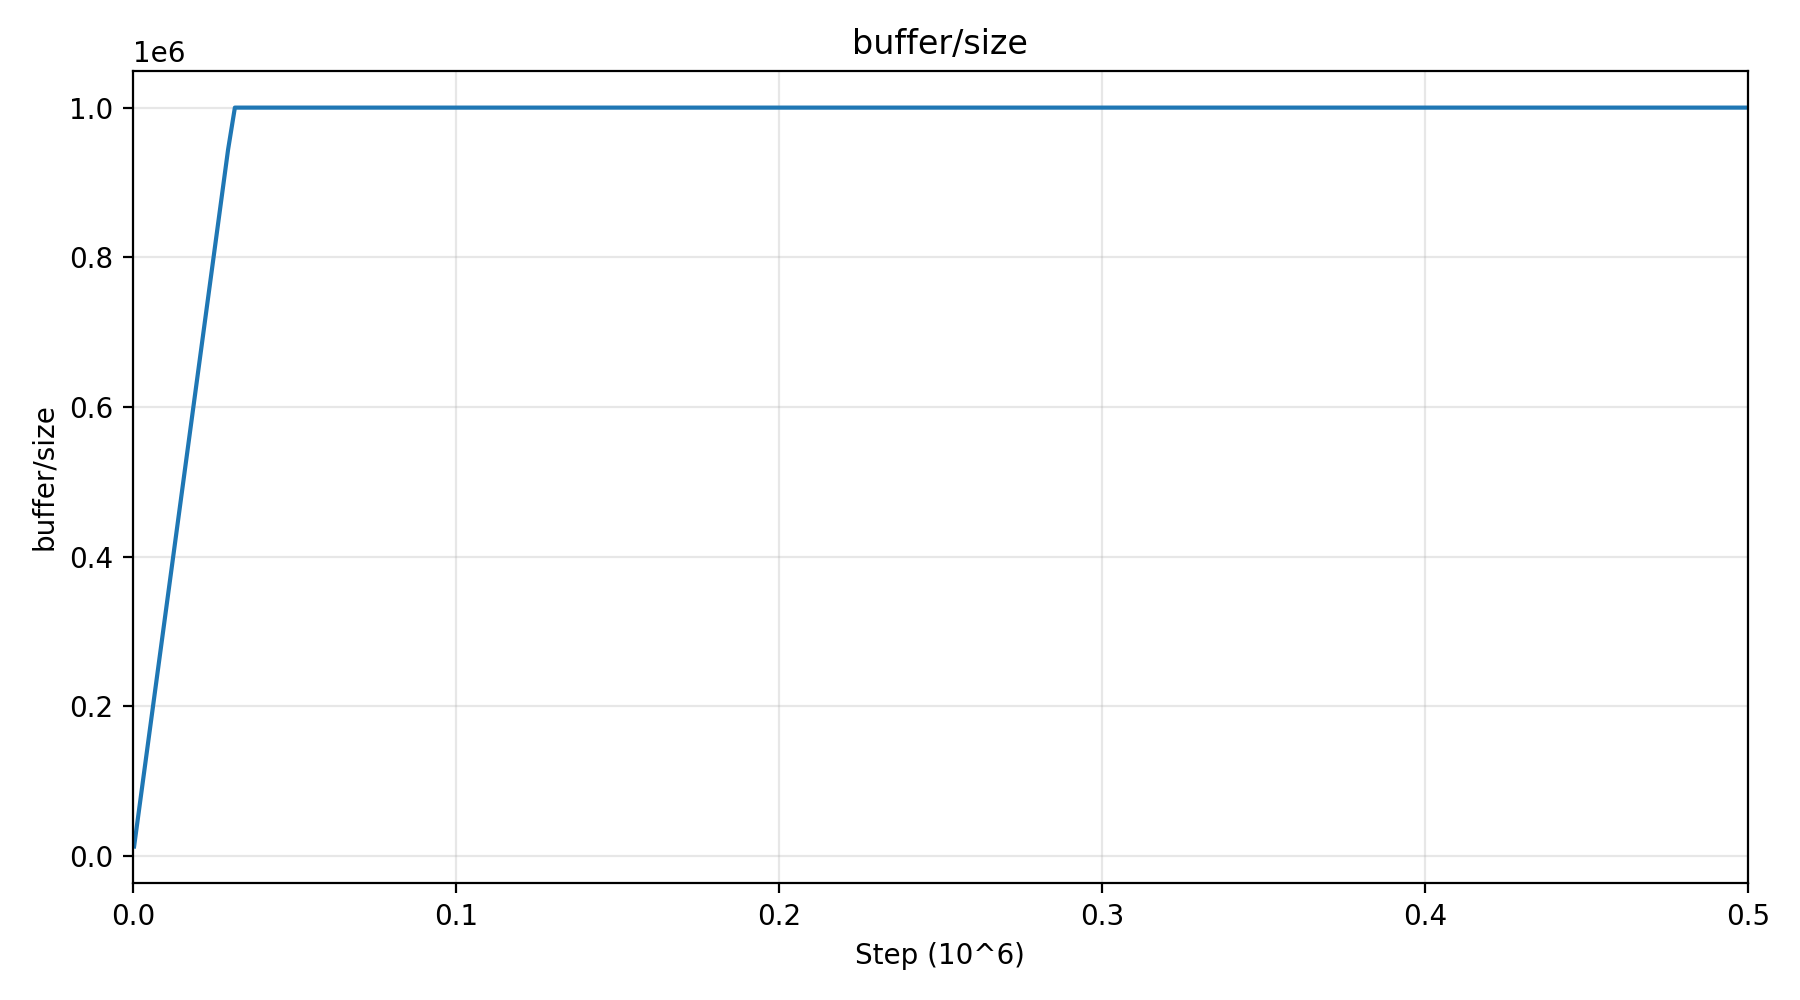
\includegraphics[width=0.5\textwidth]{figures/buffer.png}
  \caption{ASL架构性能分析}
  \label{fig:buffer-analysis}
\end{figure}
由图\ref{fig:buffer-analysis} 可见，ASL 架构的共享数据中枢在训练过程中表现出极高的稳定性与效率：在横轴（Step）的最左侧，紫线几乎是垂直向上飙升的。这表明系统在训练初期就迅速填满了经验池，达到了预设的 100 万条转移数据的容量上限。随后，经验池的占用率曲线趋于平坦，稳定在 100\% 的水平，说明系统成功实现了环形覆盖机制，同时侧面印证了ASL系统的采集数据高效性。

\section{TransSAC算法调试}

TransSAC 在 SAC 基础上引入 Transformer 编码器，使网络能够对历史状态序列进行时序建模。相比于逐帧处理，这一设计使模型能够捕捉环境动态的长期依赖，对于部分可观测环境（POMDP）下的路径规划任务尤为关键。本节介绍其核心架构与调试要点。

\subsubsection{TransSAC 网络结构}

系统维护一个长度为 $T$ 的时序窗口队列，存储最近 $T$ 个时刻的向量化观测值 $\{L(t-T+1), \dots, L(t)\}$。TransSAC 的状态表示由这一时序窗口组成 $\mathbf{s}_t = \{l_{t-T+1}, \dots, l_t\}$。

特征提取过程定义如下：先通过位置编码（Positional Encoding）为序列添加时间信息，随后经 $N_E$ 层 Transformer 编码块进行自注意力编码，最后通过全局平均池化压缩为固定维度的特征向量：

\begin{equation}
    \mathbf{z}_t = \text{AvgPool}(\text{TransformerEnc}(\mathbf{s}_t + \text{PE}))
\end{equation}

其中，$\text{PE}$ 为位置编码，$\mathbf{z}_t \in \mathbb{R}^{d_{feat}}$ 为增强后的全局特征。

Actor 与 Critic 网络分别以 $\mathbf{z}_t$ 作为输入，输出为：

\begin{align}
    \pi(a_t|s_t) &= \mathcal{N}(\mu_{\theta}(\mathbf{z}_t), \sigma_{\theta}(\mathbf{z}_t)) \\
    Q_{\phi}(\mathbf{s}_t, a_t) &= \text{MLP}_{\phi}(\text{Concat}(\mathbf{z}_t, a_t))
\end{align}

Actor 网络经过 $N_P$ 层 MLP 后输出策略分布参数；Critic 包含两个独立的 Q 网络，以实现 SAC 的双采样机制并缓解 Q 值高估。

\subsubsection{时序特征提取的优势}

与标准 SAC 相比，TransSAC 在以下方面表现出优势：

\begin{itemize}
    \item \textbf{动态环境感知}：Transformer 的自注意力机制能够自适应地学习历史状态中的关键时间步，使模型对动态障碍物的运动轨迹形成更准确的预判。
    \item \textbf{降低路径抖动}：时序上下文能够稳定策略的决策过程，避免单帧观测导致的前后不一致的动作选择。
    \item \textbf{提升样本效率}：通过编码足够的历史信息，网络能够更快地学到有效策略，整体收敛速度超过逐帧处理的方案。
\end{itemize}

\subsubsection{训练调试与超参数配置}
\begin{figure}[H]
  \centering
  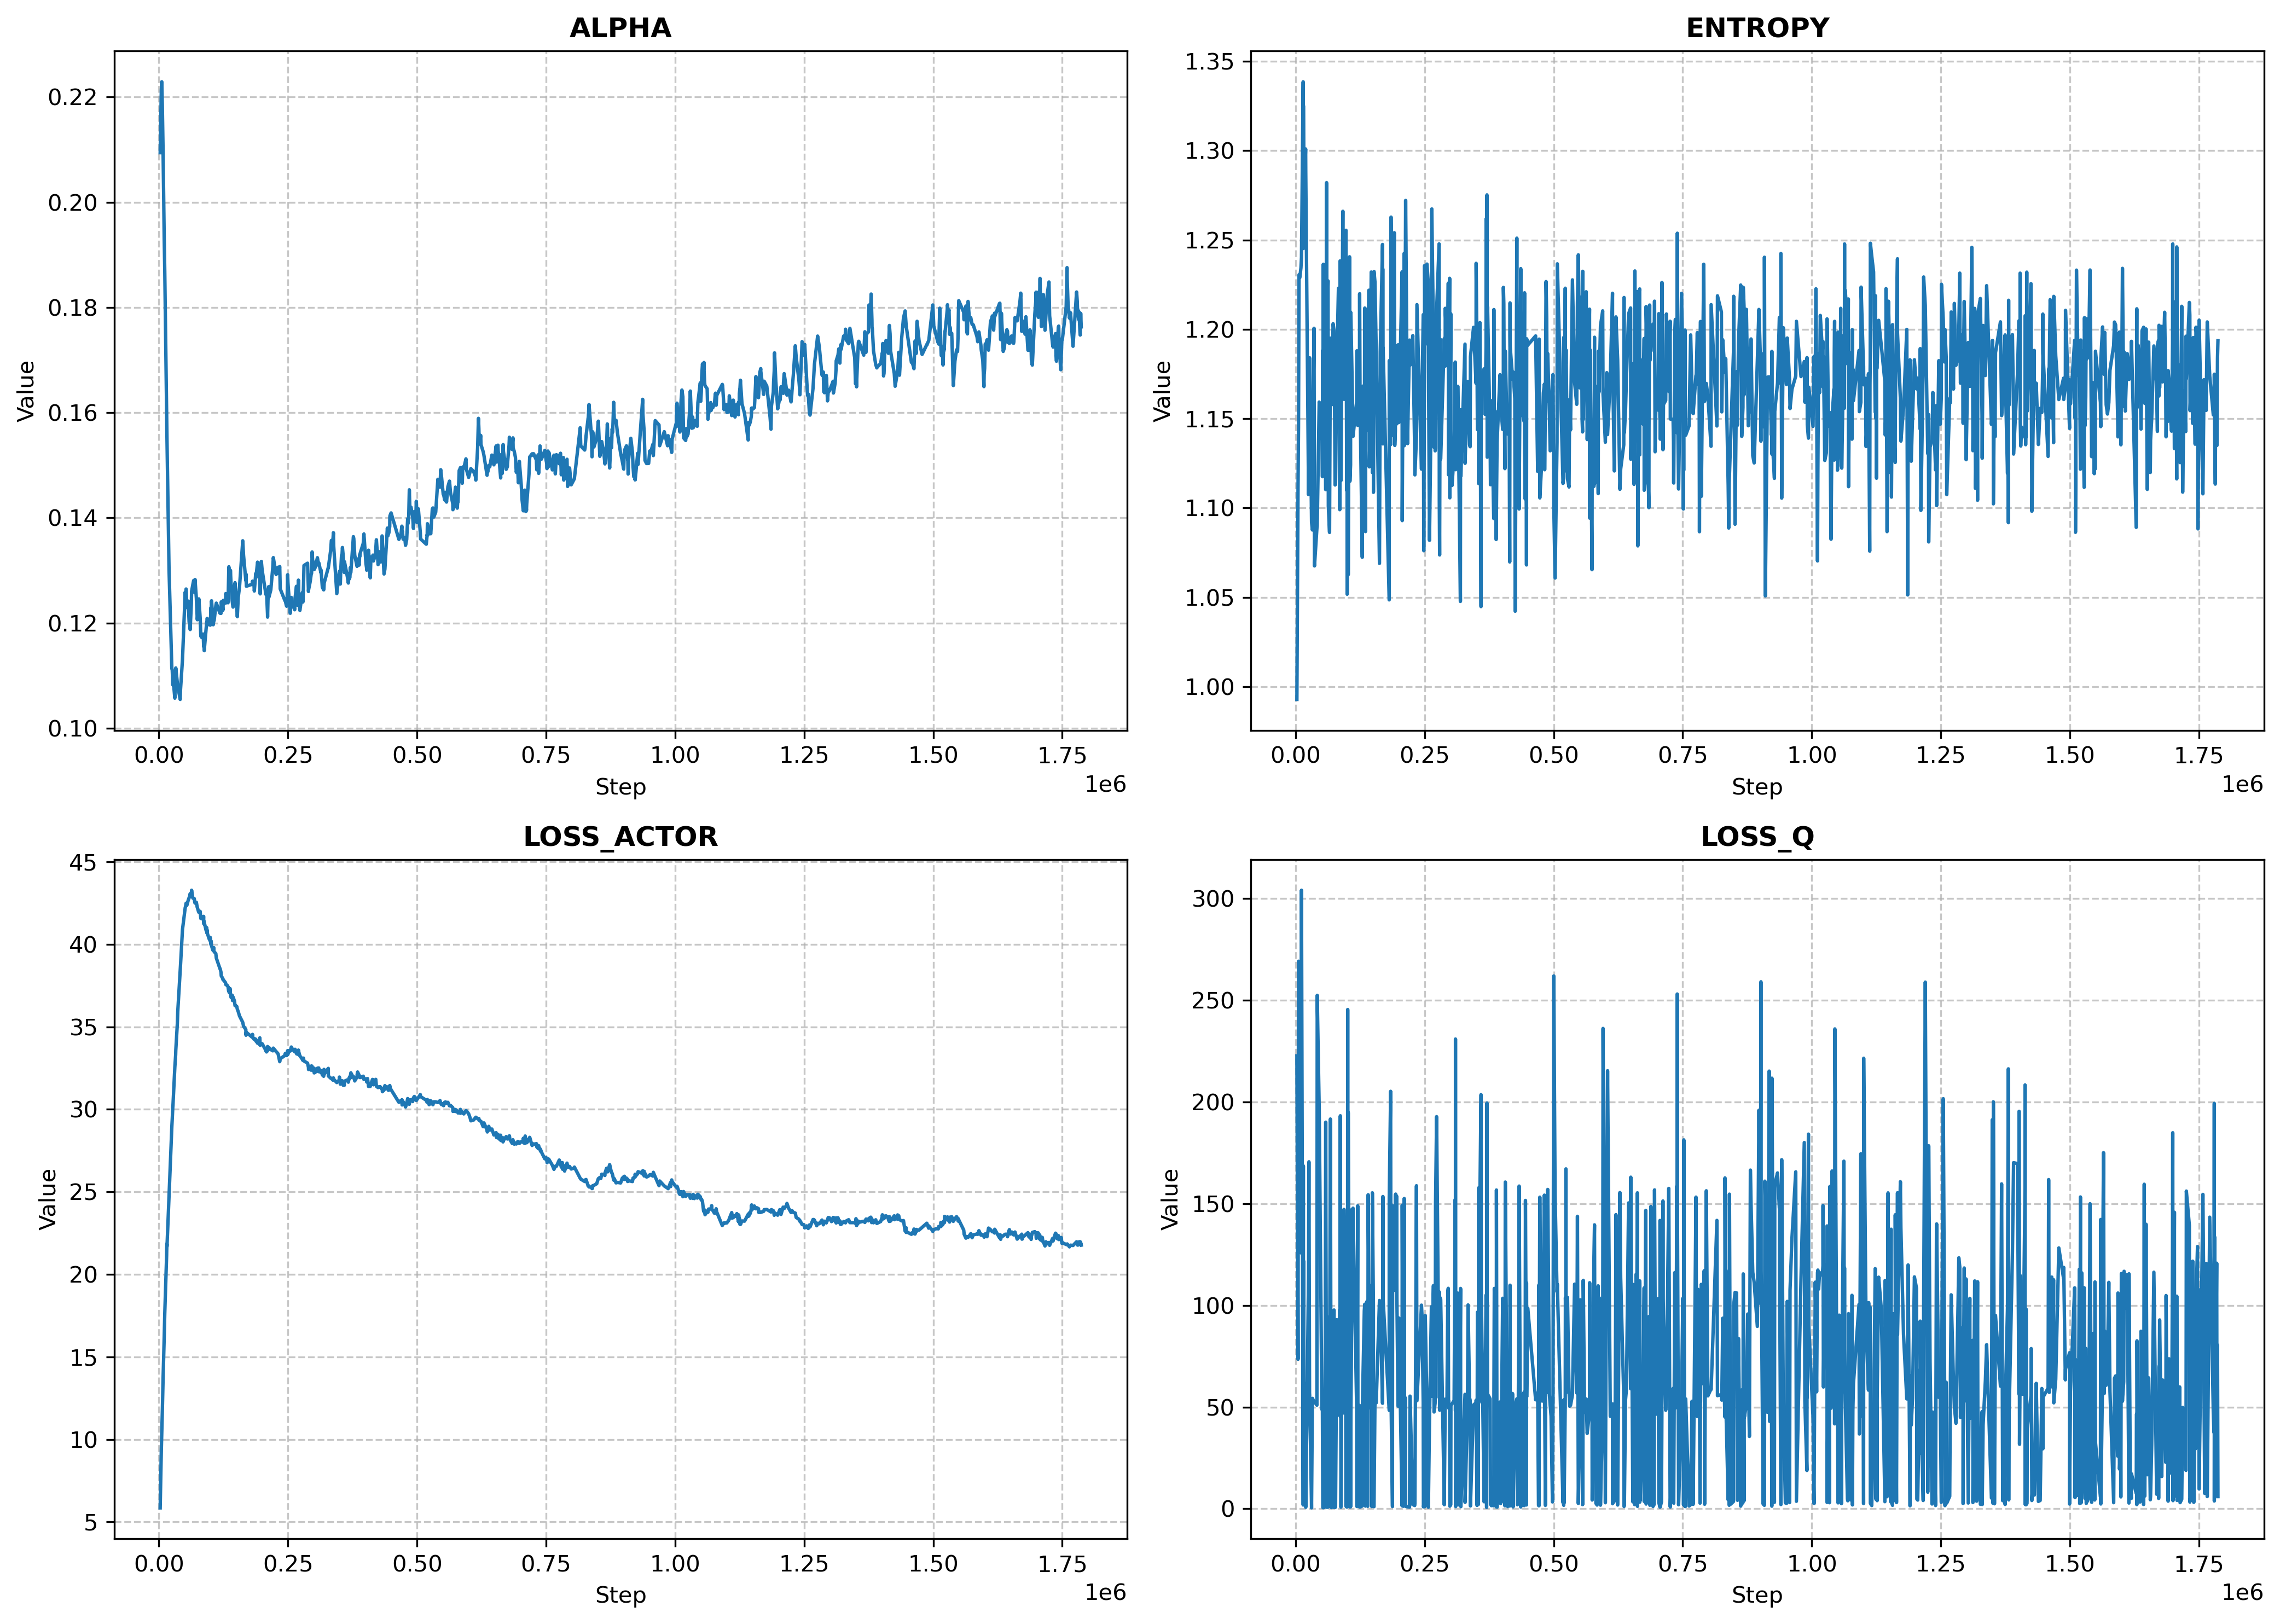
\includegraphics[width=0.7\textwidth]{figures/bad_transSAC/bad_transSAC_ASL_train_combined.png}
  \caption{TransSAC 训练中策略网络崩塌训练记录}
  \label{fig:transSAC-train-bad}
\end{figure}

\begin{figure}[H]
  \centering
  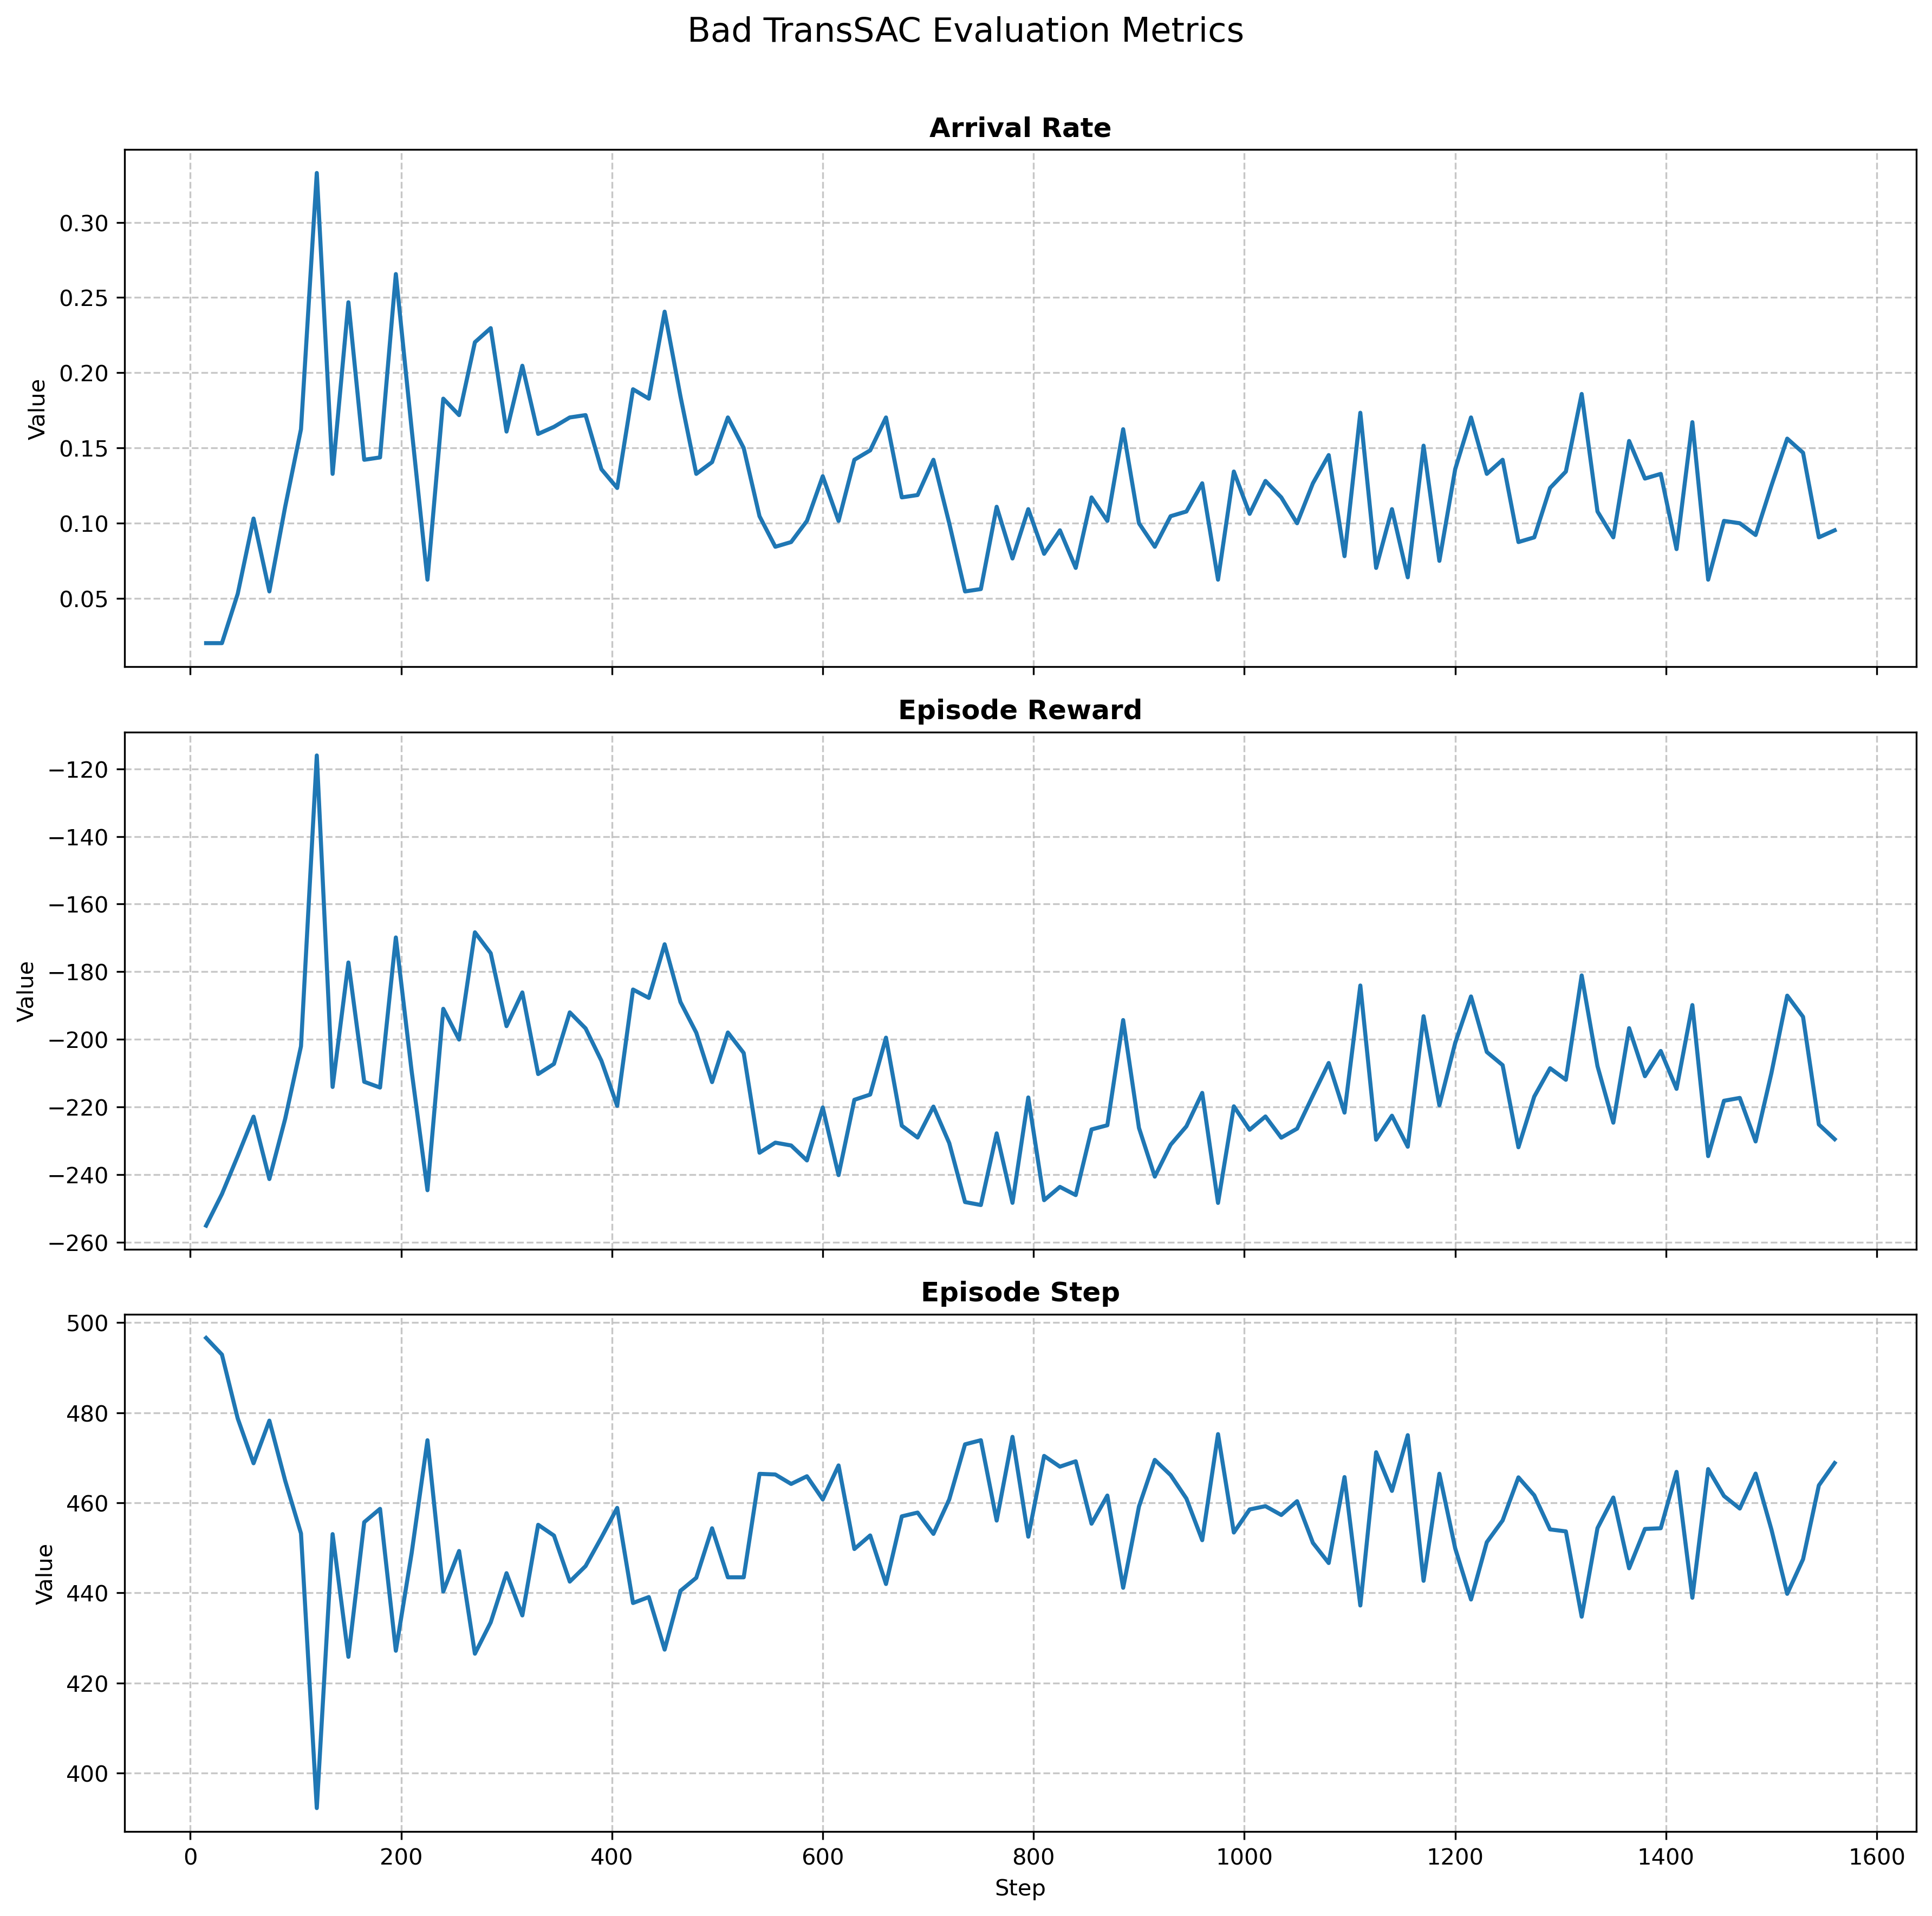
\includegraphics[width=0.7\textwidth]{figures/bad_transSAC/bad_transSAC_eval_combined.png}
  \caption{TransSAC 训练中策略网络崩塌评估结果}
  \label{fig:transSAC-eval-bad}
\end{figure}

由图\ref{fig:transSAC-train-bad} 和图\ref{fig:transSAC-eval-bad} 可见，TransSAC 在训练初期面临策略网络崩塌的挑战。这主要是由于 Transformer 层的梯度不稳定所致。训练中
ACTOR 的奖励曲线出现了剧烈的震荡，且在数千步内奖励值急剧下降至接近零的水平，表明策略网络未能有效学习到有意义的动作分布，导致智能体行为趋于随机或无效。评估结果同样显示，智能体的到达率在训练初期徘徊在 0\% 至 20\% 的低水平，且奖励值极低，进一步验证了策略网络崩塌对智能体性能的严重影响。

\subsubsection{训练失败原因分析}

图\ref{fig:transSAC-train-bad}（训练曲线）与图\ref{fig:transSAC-eval-bad}（评估记录）展示了 TransSAC 在若些实验配置下出现的策略崩塌现象：训练期内 Actor 奖励突然下降并长期徘徊在接近零的水平，评估时到达率与累计奖励也显著偏低。结合 Transformer 的结构特性与 off-policy 强化学习的训练动态，可将崩塌原因归纳为以下几点：

\begin{itemize}
    \item \textbf{自注意力层梯度尺度不稳定}：Transformer 中点积注意力在输入幅值较大或初始权重不当时，会放大梯度，导致反向传播中出现极端梯度值，从而使 Actor 或 Critic 的参数发生不稳定更新，最终触发策略退化。
    \item \textbf{训练信号的非平稳性放大}：在 off-policy 设置下，Critic 的目标依赖于自身的估计（bootstrap），若 Transformer 引入的时序特征使估计方差增大，TD 目标的振荡会被放大并反向传递到 Actor，使策略更新方向频繁改变，出现崩塌。
    \item \textbf{模型容量与样本不足不匹配}：Transformer 相对缺乏局部平移不变性（inductive bias），在样本量有限或序列长度不合适时容易过拟合局部模式或学习到无用的时序关联，从而降低泛化能力并在评估时表现为随机策略。
    \item \textbf{超参数（学习率、初始化、归一化）敏感性}：Transformer 对学习率和参数初始化特别敏感，过大的学习率或缺乏学习率预热会使注意力层在训练早期产生巨大权重更新；此外 LayerNorm 的位置（PreNorm vs PostNorm）与是否使用残差缩放也会影响梯度传播稳定性。
    \item \textbf{Actor–Critic 失衡}：若 Critic 学习过慢或过快，相对于 Actor 出现偏差，Actor 可能根据错误的价值估计进行更新，导致策略性能退化并最终塌陷为低质量随机策略。
\end{itemize}

以上几方面往往交织导致训练崩塌；因此调试时需同时从网络结构、优化器与训练调度三类维度入手。

\subsubsection{超参数调整与调试流程}

针对上述崩塌原因，本文采取了系统化的调试流程，按优先级逐步试验并验证效果，关键步骤与建议配置如下：

\begin{enumerate}
    \item \textbf{重现问题并保存快照}：在未改动超参数前，先保存发生崩塌的训练日志、模型快照与经验回放样本，用于后续对比与回滚。

    \item \textbf{梯度裁剪与学习率预热}：立即引入全局范数裁剪（例如 $\text{clip\_norm}=1.0$）并对 Transformer 子模块单独设置较小的学习率（例如 $\mathrm{lr}_{\mathrm{trans}}=1\times10^{-4}$），对整个训练过程采用学习率预热（warmup）策略（例如 warmup 2000 步），以抑制初期极端梯度。优化器建议使用 AdamW 并加上小量权重衰减（例如 $1\times10^{-4}$）。

    \item \textbf{简化 Transformer 结构以降低不稳定性}：将编码器层数从较深的 $N_E$ 降至 $1\sim2$ 层，或减小特征维度 $d_{feat}$（例如 128），并启用 0.1 的 dropout，以降低过拟合风险与梯度波动幅度。

    \item \textbf{改用 Pre-LayerNorm 与残差缩放}：把 LayerNorm 放在子层前（PreNorm），该做法在深层 Transformer 中常能显著改善梯度流动稳定性；必要时在残差分支上加上缩放因子（例如 $1/\sqrt{2}$）以抑制跳变。

    \item \textbf{调整序列长度与批量大小}：若序列窗口 $T$ 过长会提高方差，推荐从 $T=8$ 逐步缩短到 $T=4$ 或 $T=6$ 做对比；同时适当增大批量（例如 $B=256$）可降低梯度噪声，配合较小的学习率通常能提升稳定性。

    \item \textbf{平衡 Actor 和 Critic 的更新频率}：增大 Critic 的更新步数或使用更频繁的目标网络同步（例如 target \tau=0.005，target update 每 1k 步），并调整 UTD（Update-To-Data）比率至 $2\sim4$，以减少价值估计的高方差对 Actor 的冲击。

    \item \textbf{正则化与归一化}：对输入特征执行逐维标准化（mean-std），对 Transformer 添加 weight decay（AdamW）和 dropout，以抑制过拟合并减小训练振荡。

    \item \textbf{监控与自动回退}：实现训练指标的实时监控（Actor reward、Critic loss、TD error 的滑动均值），若发现 Critic loss 或 TD error 出现异常陡增，则自动降低学习率或回退至上一次稳定快照。

    \item \textbf{最终验证与对比}：在每次超参数组调整后，使用固定的验证场景集（例如 100 次独立种子）评估到达率、平均步数与平均奖励，确保所做改动在泛化评估中带来实质性改善而非训练集过拟合。
\end{enumerate}

按上述流程逐项排查并调整，最终训练收敛，评估结果如下：

TransSAC 的训练过程与 SAC 保持一致，主要区别在于时间窗口长度 $T$ 的选择。在本文实验中，设定 $T=8$ 步作为短期上下文窗口，既能捕捉障碍物的动向，又不会过度增加计算延迟。此外，为防止 Transformer 层数过多导致梯度消失，本文采用了 $N_E=2$ 层编码块与 LayerNorm 正则化相结合的轻量级设计。

在训练初期，遇到过网络极易崩溃的问题，原因是transformer层的梯度不稳定。通过引入梯度裁剪（Gradient Clipping）和学习率预热（Learning Rate Warmup）策略，成功稳定了训练过程，使得 TransSAC 能够在数千步内达到初始性能水平。


相比单纯 SAC，TransSAC 的训练初期即表现出更稳定的到达率（约 50\%），说明时序建模确实带来了决策质量的提升。在后续验证对比中，这一架构的优势将被进一步量化。

\begin{figure}[H]
  \centering
  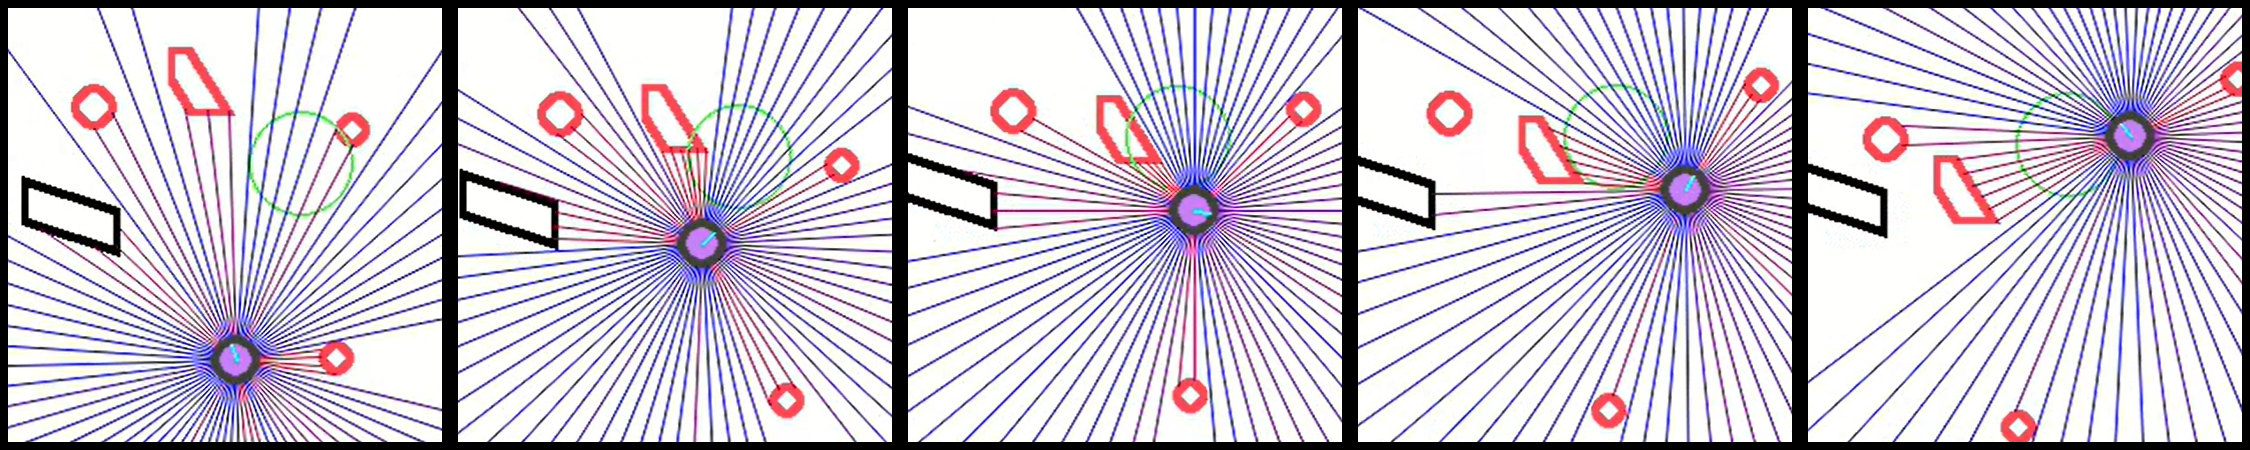
\includegraphics[width=0.7\textwidth]{figures/experiment1_stitched.png}
  \caption{TransSAC 训练中智能体学到的高级避障技能展示（序列1）}
  \label{fig:action_1}
\end{figure}

\begin{figure}[H]
  \centering
  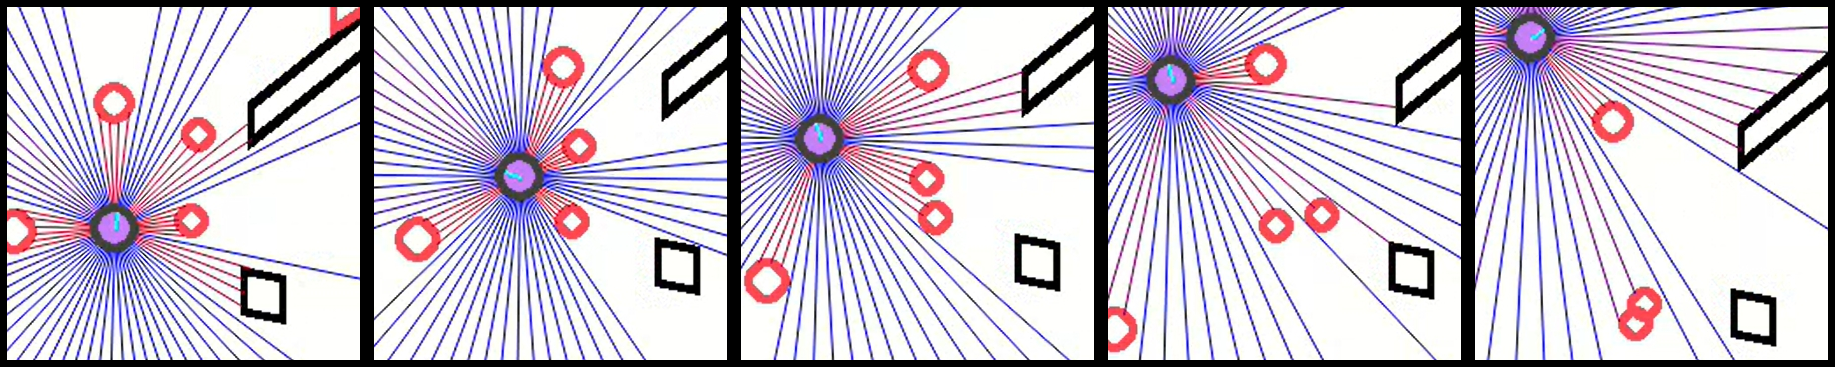
\includegraphics[width=0.7\textwidth]{figures/experiment2_stitched.png}
  \caption{TransSAC 训练中智能体学到的高级避障技能展示（序列2）}
  \label{fig:action_2}
\end{figure}

\begin{figure}[H]
  \centering
  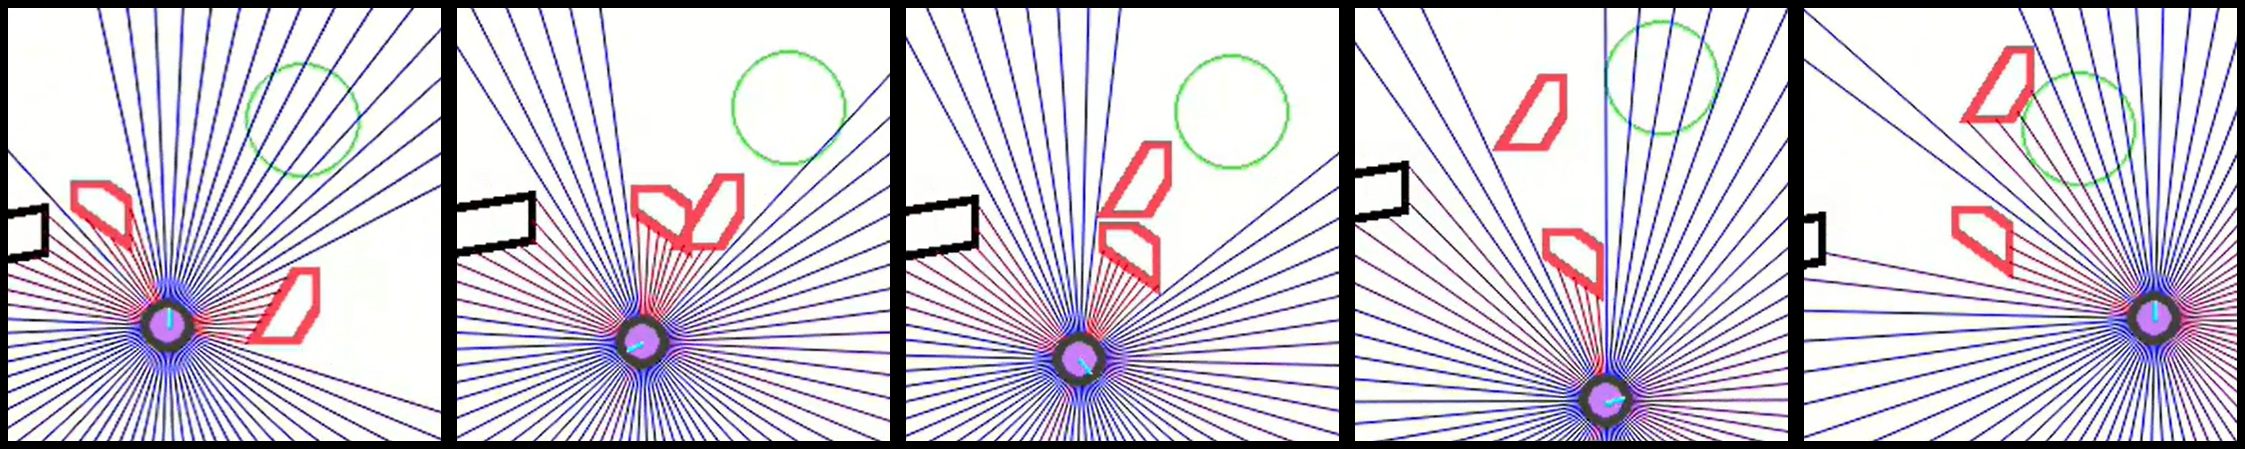
\includegraphics[width=0.7\textwidth]{figures/experiment3_stitched.png}
  \caption{TransSAC 训练中智能体学到的高级避障技能展示（序列3）}
  \label{fig:action_3}
\end{figure}

从上述实验序列可以看出，经过充分训练的 TransSAC 智能体学会了对动态障碍物的主动闪避、等待等在复杂环境中的路径优化的高级导航技能。
\section{路径规划算法对比}

\begin{figure}[H]
  \centering
  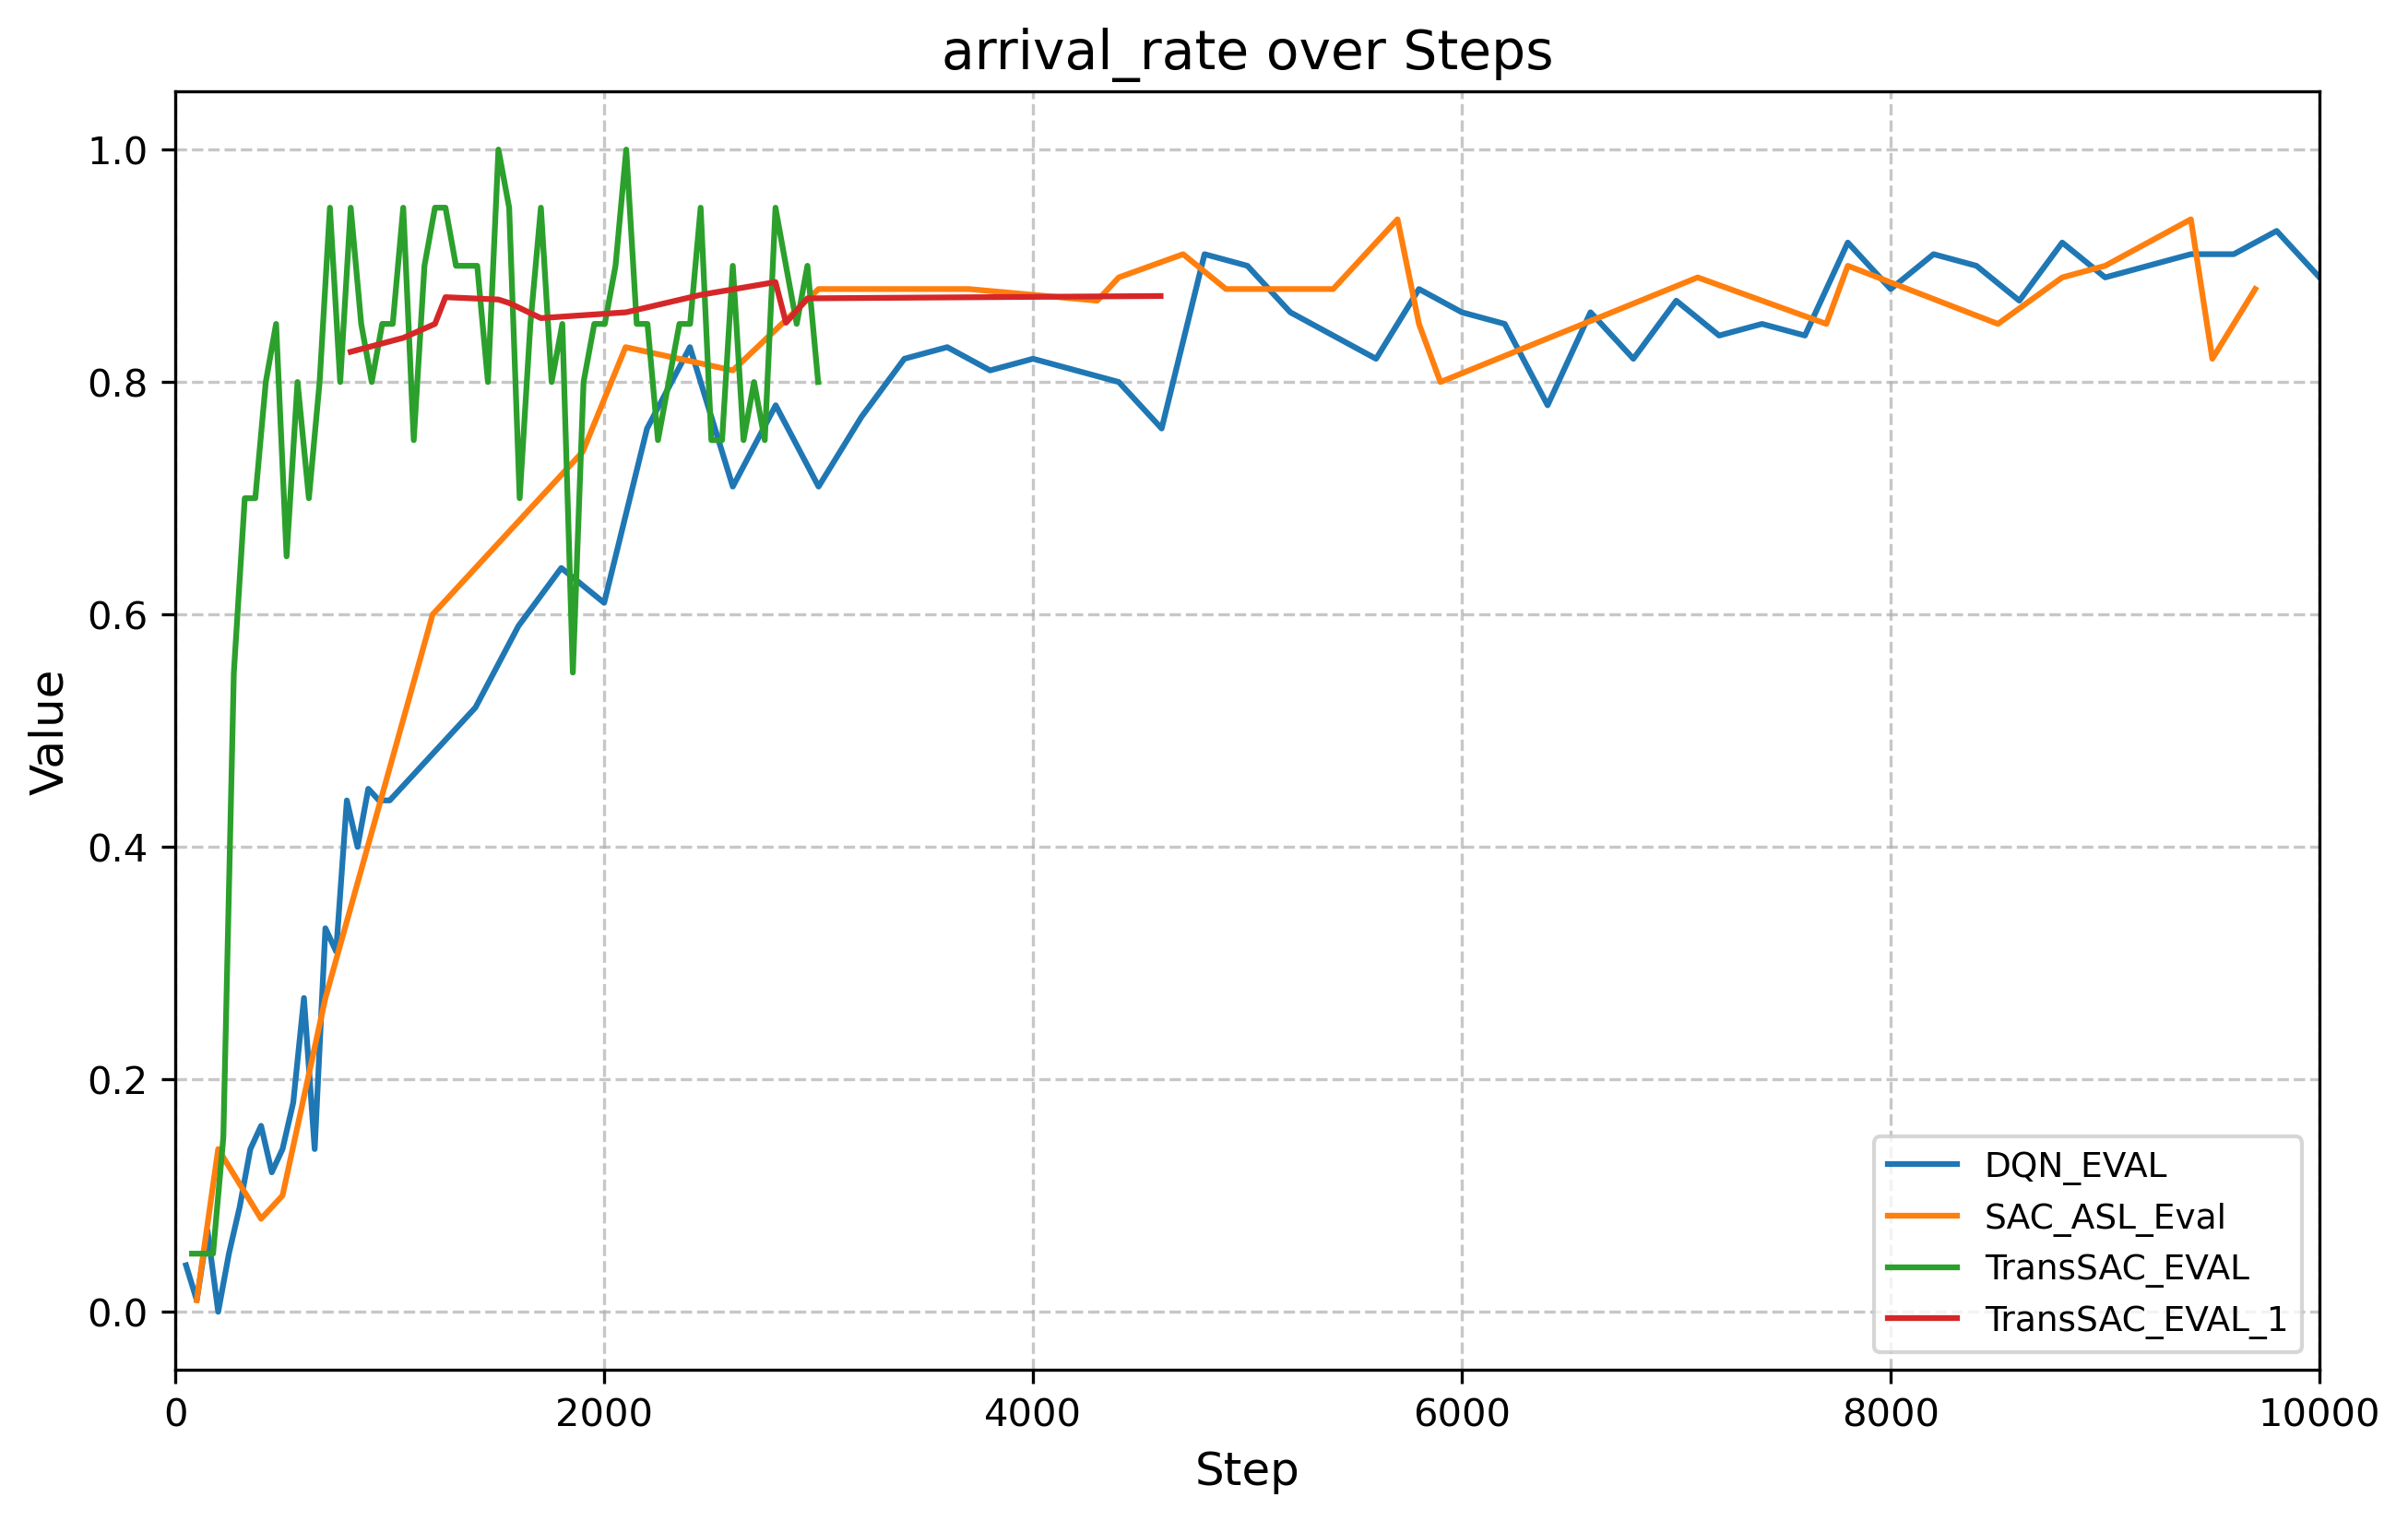
\includegraphics[width=0.7\textwidth]{figures/comparison/arrival_rate.png}
  \caption{到达率对比}
  \label{fig:comparison_arrival_rate}
\end{figure}

\begin{figure}[H]
  \centering
  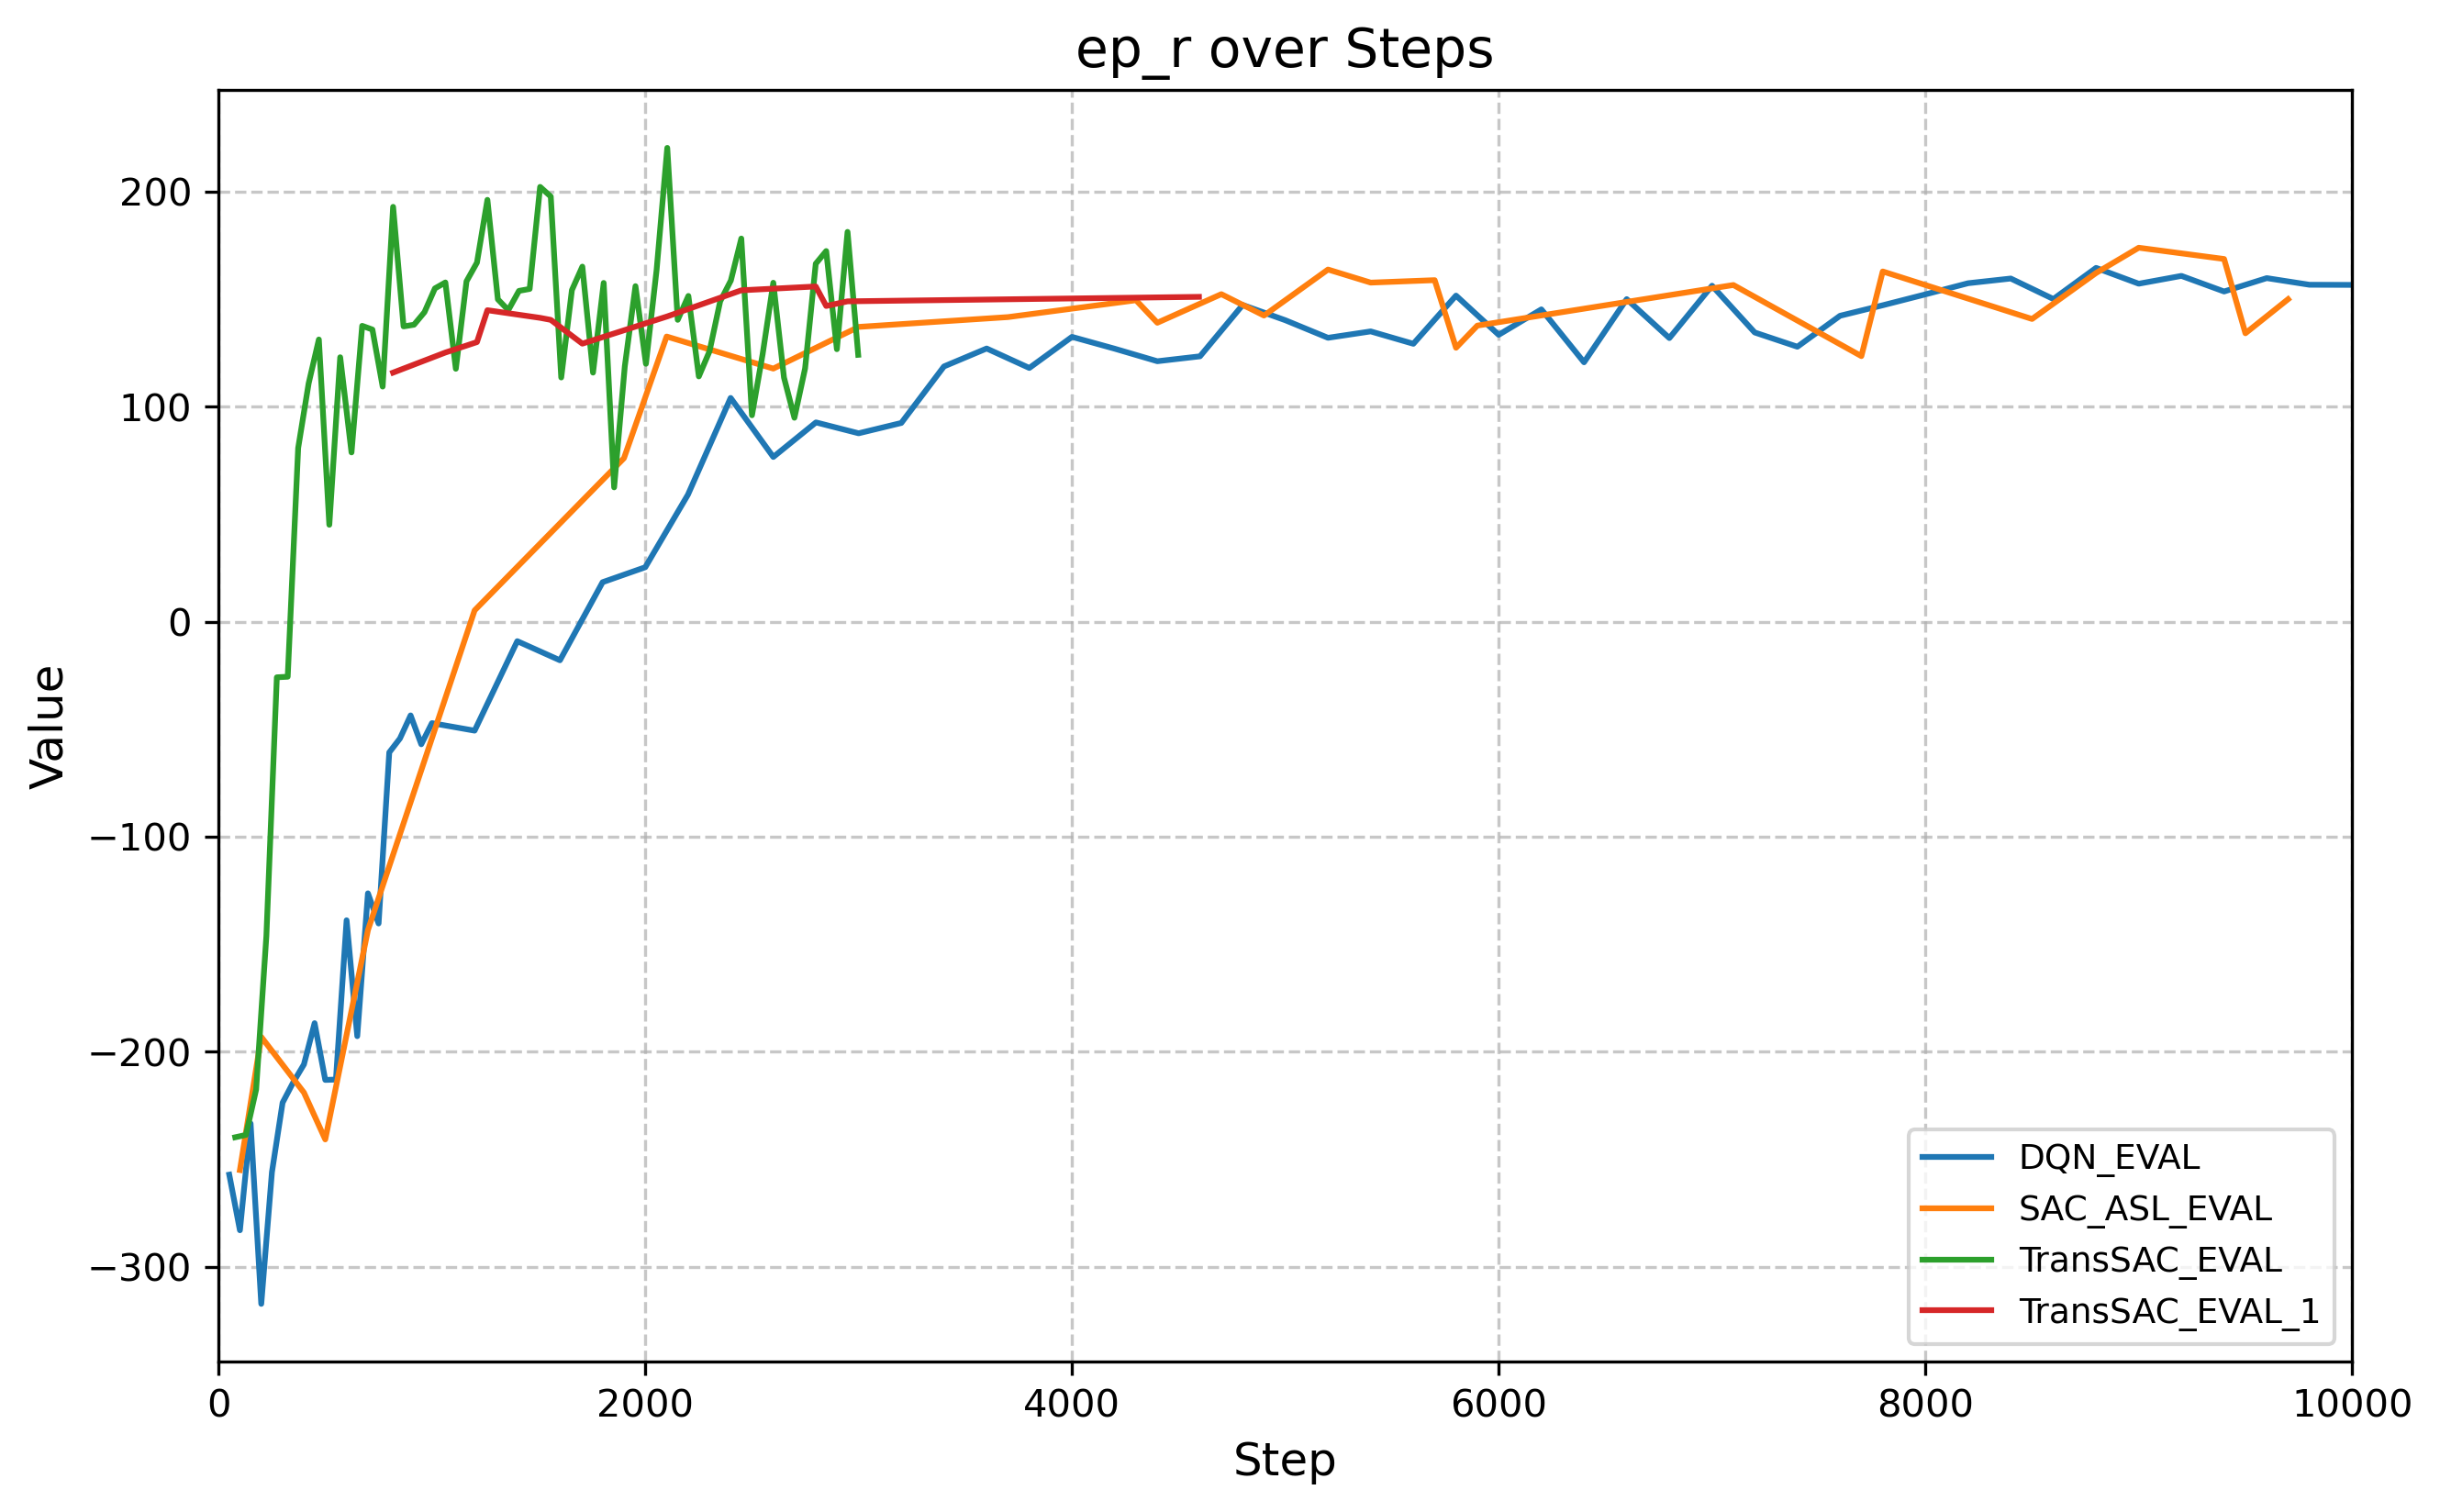
\includegraphics[width=0.7\textwidth]{figures/comparison/ep_r.png}
  \caption{累积奖励对比}
  \label{fig:comparison_ep_r}
\end{figure}

\begin{figure}[H]
  \centering
  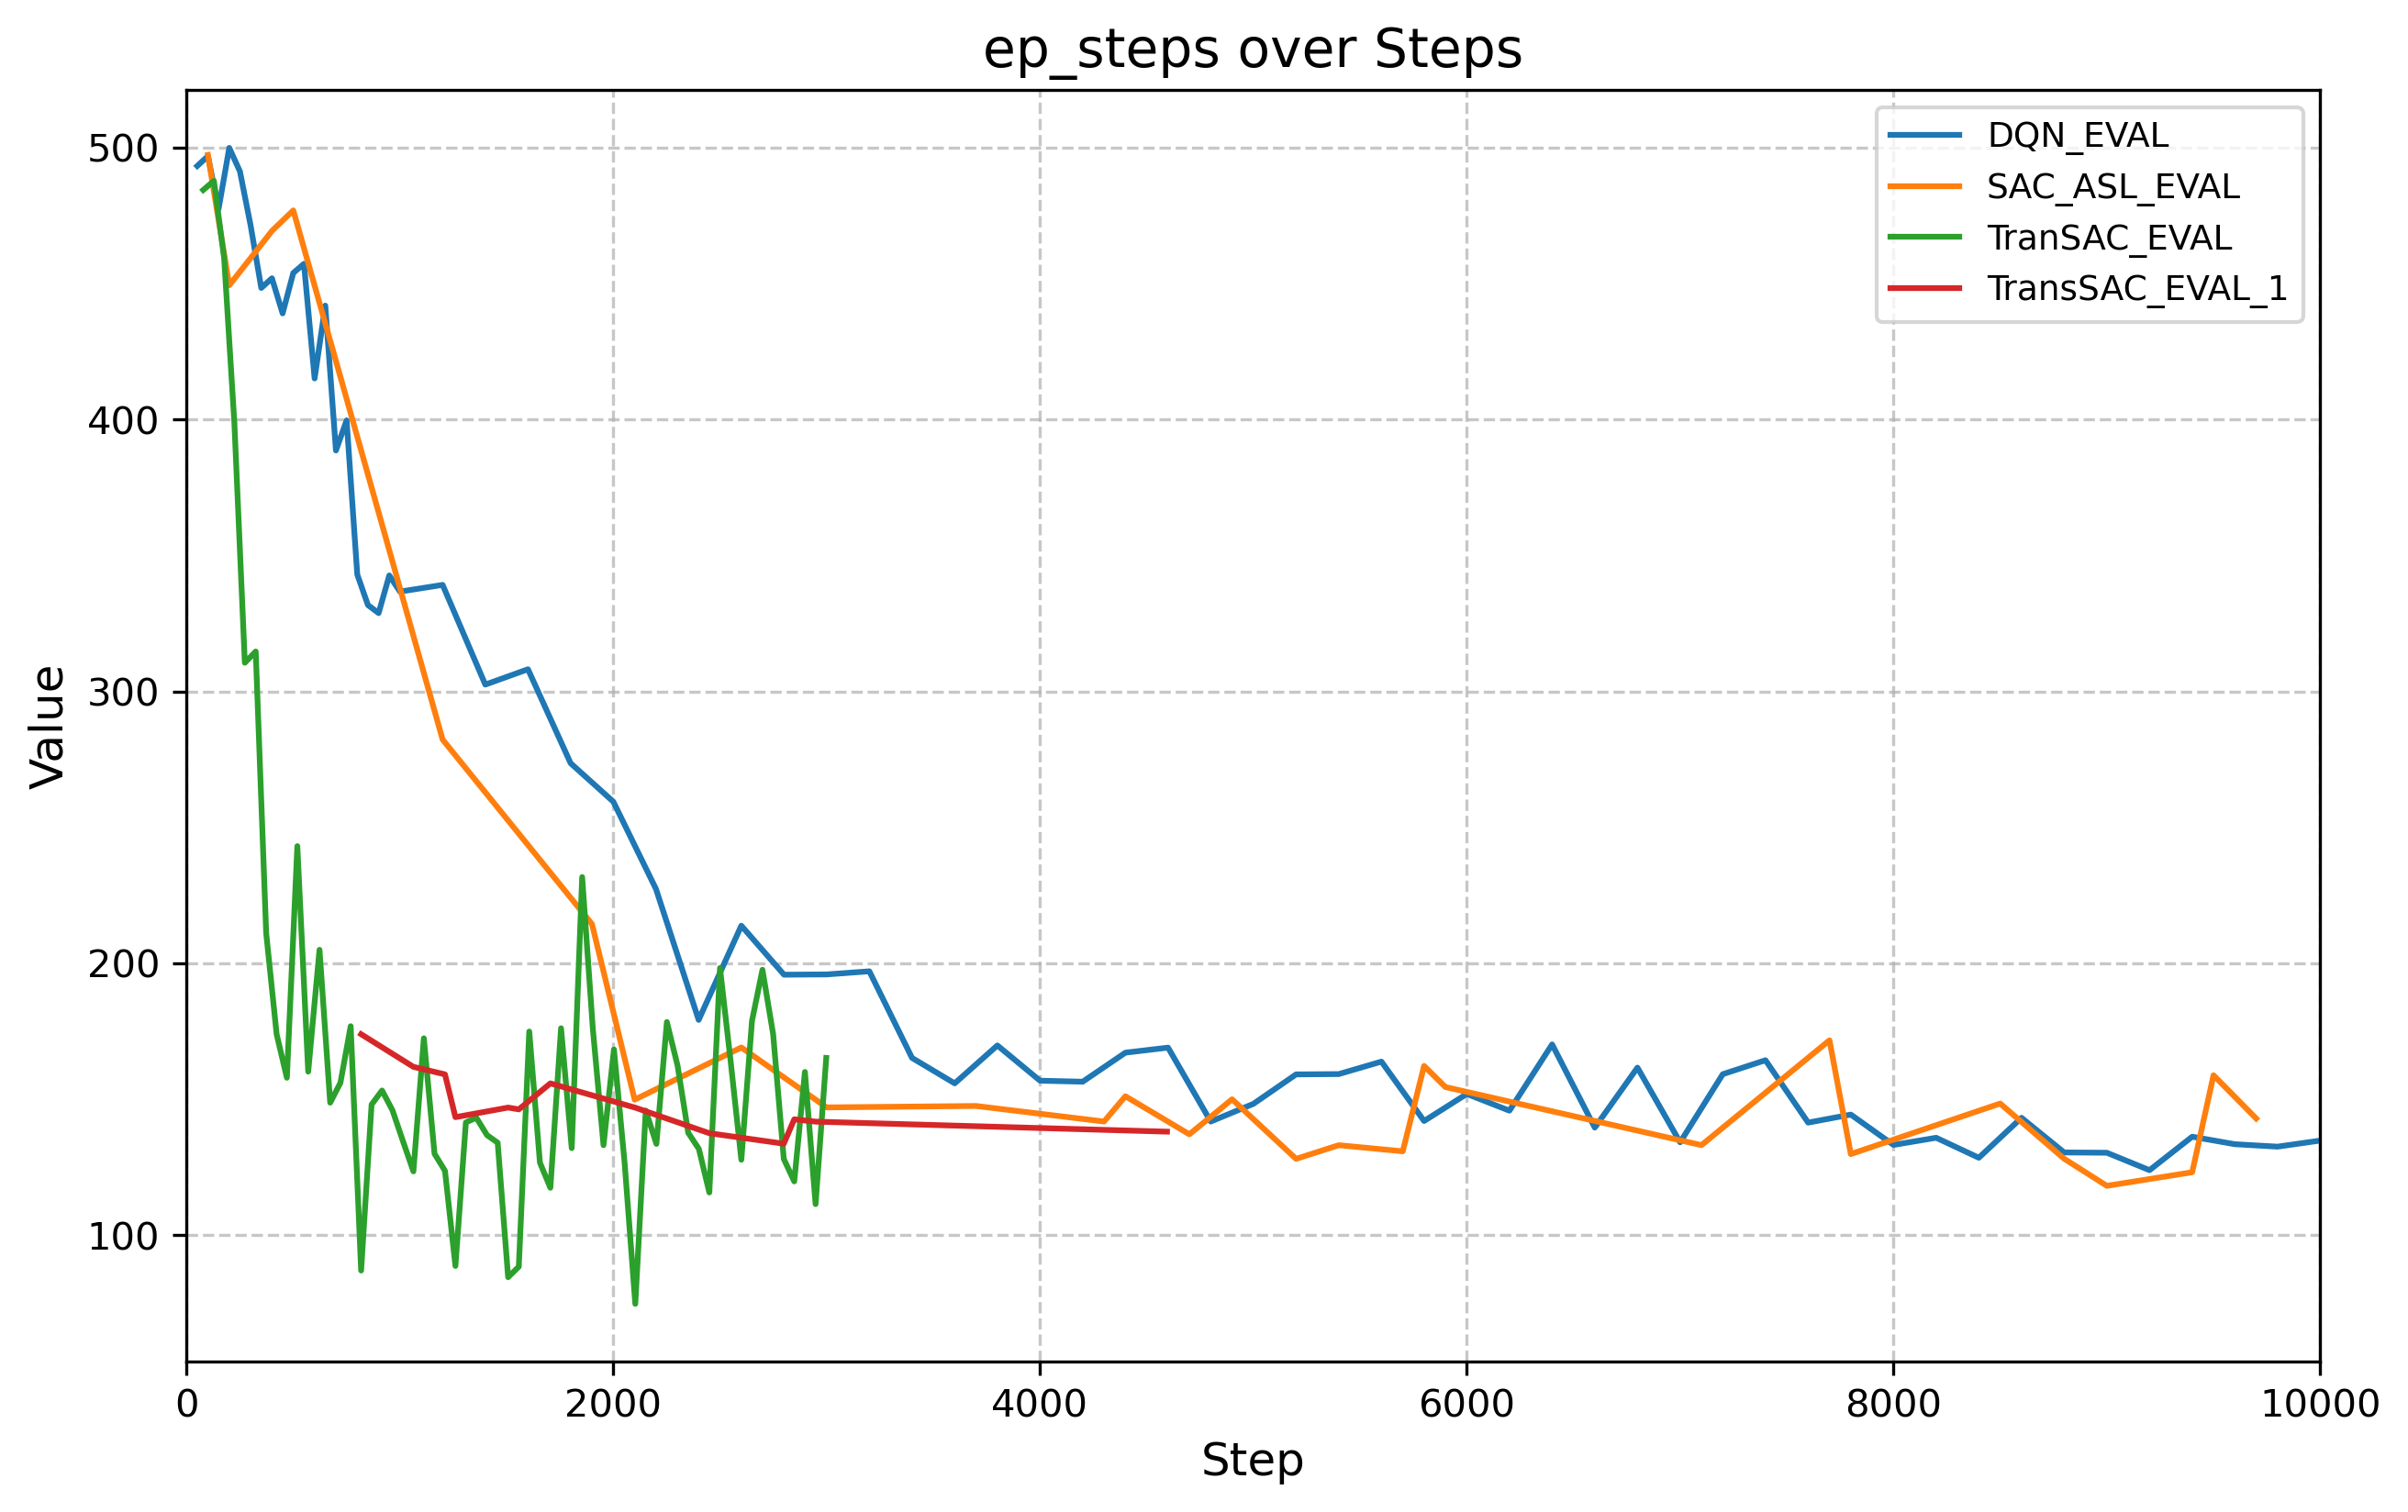
\includegraphics[width=0.7\textwidth]{figures/comparison/ep_steps.png}
  \caption{路径长度对比}
  \label{fig:comparison_ep_steps}
\end{figure}